% OFFROAD-REPORT template for LaTeX
% offroad-example.tex
% Originally created by Joshua A. Marshall on 11 July 2013

% Set document parameters (font, paper, eqn position, page style)
\documentclass[12pt,letterpaper,fleqn,oneside,titlepage]{offroad-report}

% ---------------------------------------------------------------

% Some math packages that give you more symbols
\usepackage{amssymb,amsfonts,amsmath,amscd}

\usepackage{nccmath}

\usepackage{pifont}

% A package that allows easy input of web URLs.
\usepackage{url}

% For underlining stuff in a nice way
\usepackage[normalem]{ulem}

% For verbatim stuff, like simple code
\usepackage{verbatim}

% For better looking tables
\usepackage{booktabs}

% For cover page wallpaper
\usepackage{wallpaper}

% For better bold maths
\usepackage{bm}

% For subfig
\usepackage{graphicx}
\usepackage{subfig}

% For link
\usepackage{hyperref}
\hypersetup{
    colorlinks=true,
    linkcolor=black,
    filecolor=black,      
    urlcolor=blue,
}
% ---------------------------------------------------------------

% Some handy commands
\newcommand{\norm}[1]{\left\Vert#1\right\Vert}
\newcommand{\abs}[1]{\left\vert#1\right\vert}
\newcommand{\set}[1]{\left\{#1\right\}}
\newcommand{\Real}{\mathbb R}
\newcommand{\Complex}{\mathbb C}
\newcommand{\eps}{\varepsilon}
\newcommand{\To}{\longrightarrow}
\newcommand{\Ker}{\textup{Ker}}
\newcommand{\Img}{\textup{Img}}
\newcommand{\diag}{\textup{diag}}
\newcommand{\circulant}{\textup{circ}}
\newcommand{\mbf}{\bm}

% ---------------------------------------------------------------

% Define some hyphenation (add whatever you want)
\hyphenation{aero-space} \hyphenation{auton-omous}

% ---------------------------------------------------------------

\begin{document}

% Set the page style for the document
\pagestyle{plain}

% ---------------------------------------------------------------

% Set the title stuff (make title bold, put address, today's date)
\title{\bf An Intuitive Tutorial to Gaussian Processes Regression}
\author{Jie Wang \\ 
        Ingenuity Labs Research Institute \\ 
        \texttt{jie.wang@queensu.ca}}
\date{\today}

% Make the title page
\maketitle
\thispagestyle{empty}

% Insert a logo and address
\begin{center}

\includegraphics[width=1.5in]{figs/offroad-icon.pdf} \\ \vspace{12pt}
\large
Offroad Robotics \\
c/o Ingenuity Labs Research Institute \\ 
Queen's University \\
Kingston, ON K7L 3N6 Canada
\end{center}

% Add the Ingenuity Labs wallpaper
\ThisCenterWallPaper{1.0}{figs/ingenuity-labs-cover.pdf}

% Make the first page empty (no headers, footers)
\thispagestyle{empty}

% ---------------------------------------------------------------

% Abstract
\newpage
\thispagestyle{empty}
\begin{abstract}
This introduction aims to provide readers an intuitive understanding of Gaussian processes regression. Gaussian processes regression (GPR) models have been widely used in machine learning applications because their representation flexibility and inherently uncertainty measures over predictions. The paper starts with explaining mathematical basics that Gaussian processes built on including multivariate normal distribution, kernels, non-parametric models, joint and conditional probability. The Gaussian processes regression is then described in an accessible way by balancing showing unnecessary mathematical derivation steps and missing key conclusive results. An illustrative implementation of a standard Gaussian processes regression algorithm is provided. Beyond the standard Gaussian processes regression, existing software packages to implement state-of-the-art Gaussian processes algorithms are reviewed. Lastly, more advanced Gaussian processes regression models are specified. The paper is written in an accessible way, thus undergraduate science and engineering background will find no difficulties in following the content. 
\end{abstract}

% ---------------------------------------------------------------

% Add a table of contents (comment out if you want to remove)
\newpage
\thispagestyle{empty}
\tableofcontents

% ---------------------------------------------------------------

% Reset the page numbering
\newpage
\setcounter{page}{1}

% ---------------------------------------------------------------
\section{Introduction}

The Gaussian processes is a probabilistic supervised machine learning framework that has been widely used for regression and classification tasks. The Gaussian processes regression (GPR) model can make predictions incorporating prior knowledge (kernels) and provide uncertainty measures over predictions \cite{Rasmussen2006}. Besides signal processing \cite{fuentes2020autonomous}, GPR is actively used for dynamic system model estimations in reinforcement learning \cite{Deisenroth2015} and control \cite{Ostafew2016}. GPR can provide uncertainty estimations not only for one-step prediction but also for multi-step predictions by propagating the uncertainty multi-step ahead \cite{Girard2002}. Due to its ability of multi-step uncertainty propagation, GPR is increasingly applied together with model predictive control (MPC) in the past several years \cite{Hewing2020}. The strength of using GPR is that it can model the unmodeled dynamics and unknown disturbances that are hard to model by the first principle method. More importantly, the GPR model quantifies uncertainty during the model learning to indicate areas with less certain to be explored more. An efficient implementation of GPR makes online learning possible to control tasks \cite{Kabzan2019}. 

Gaussian processes model is a supervised learning method mainly developed within the computer science and statistics communities. Researchers with engineering backgrounds often find it's difficult to gain a clear understanding of GPR easily. To understand GPR, even to the intuitive level, needs to have mathematics foundation knowledge including multivariate normal distribution (MVN), kernels, non-parametric model, and joint and conditional probability. There is often a gap between using GPR as a tool and feeling comfortable to use it due to the difficulties in understanding these necessary theories. This introduction aims to bring readers an intuitive understanding of GPR in an accessible way. All implementation codes in this paper are provided at: \url{https://github.com/jwangjie/An-Intuitive-Tutorial-to-Gaussian-Processes-Regression}. 

\section{Mathematical Basics}
This section covers the mathematical basics that GPR models are built on. It starts with Gaussian (normal) distribution, then goes through multivariate normal distribution (MVN), kernels, non-parametric model, and joint and conditional probability. In order to obtain a clear understanding of GPR, unnecessary math is neglected on purpose. First of all, what is regression? Regression is a common machine learning task that is described as given some observed data points, fitting a function that represents these data point features, then using the function to make predictions at new data points. For a given set of observed data points shown in Fig. \ref{FIG:1}(a), there are infinite numbers of possible functions that fit the data points. In Fig. \ref{FIG:1}(b), we show five samples of potential infinite numbers of functions that fit the data points in Fig. \ref{FIG:1}(a). 
\begin{figure}[h!]
    \centering
    \subfloat[Data point observations]{{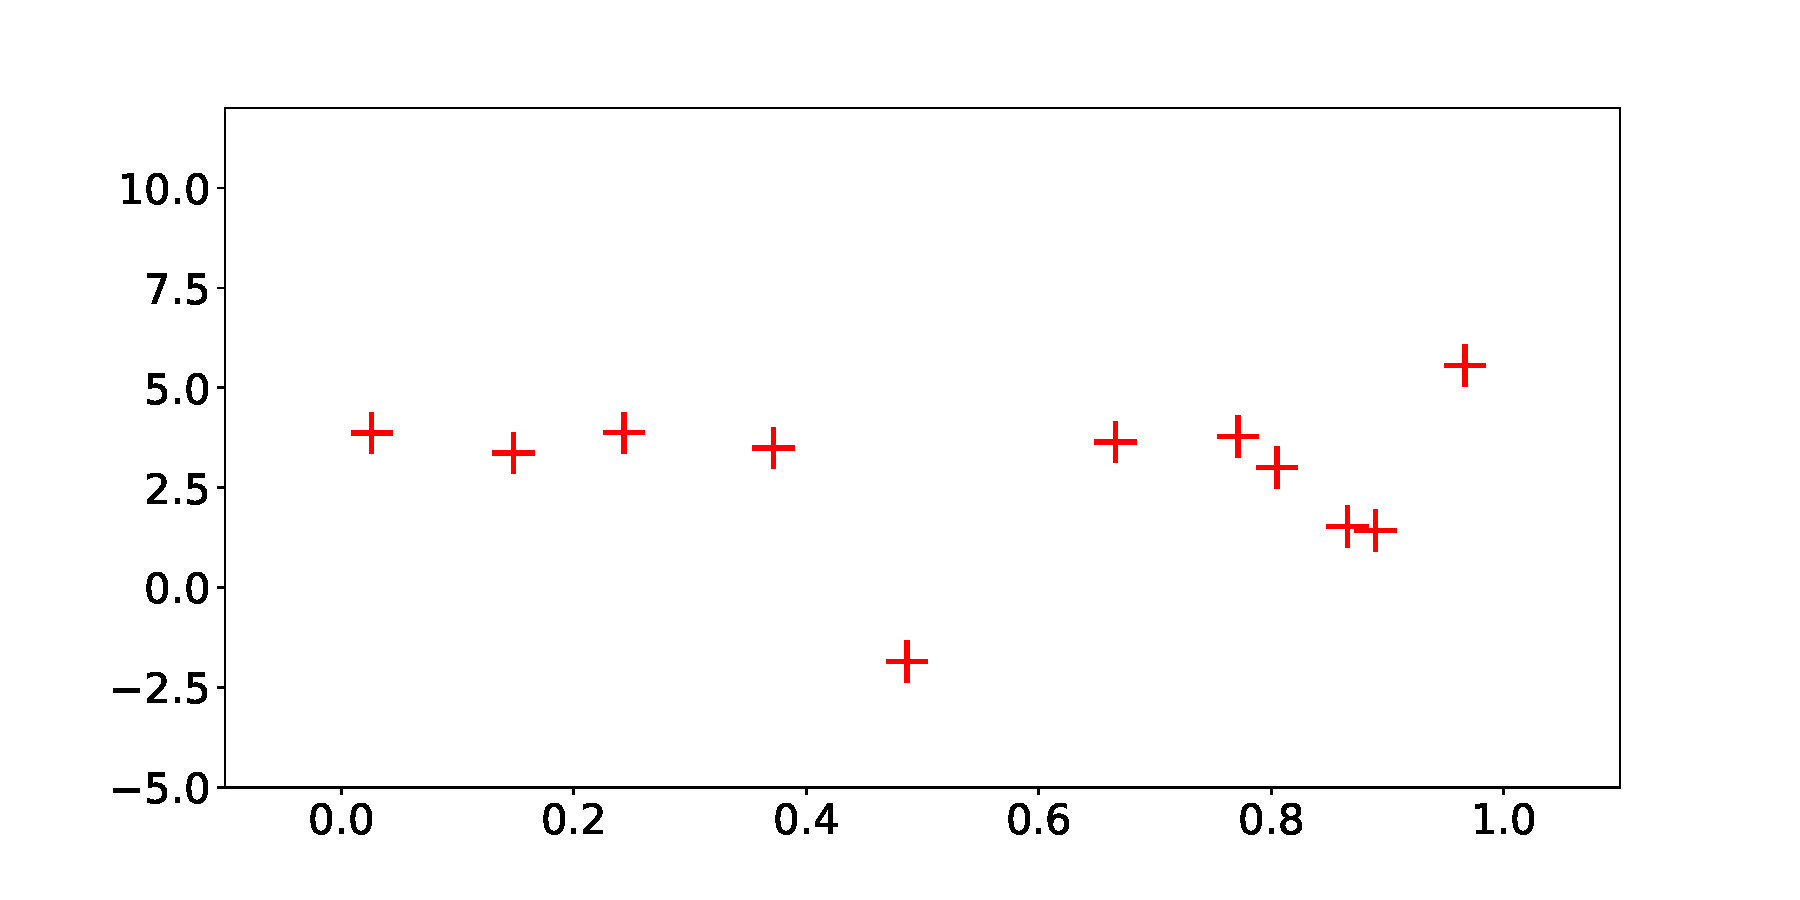
\includegraphics[trim=2.0cm 0.8cm 3.2cm 1.8cm, width=7.0cm]{figs/regression_points.pdf} }}
    \qquad
    \subfloat[Five possible regression functions by GPR]{{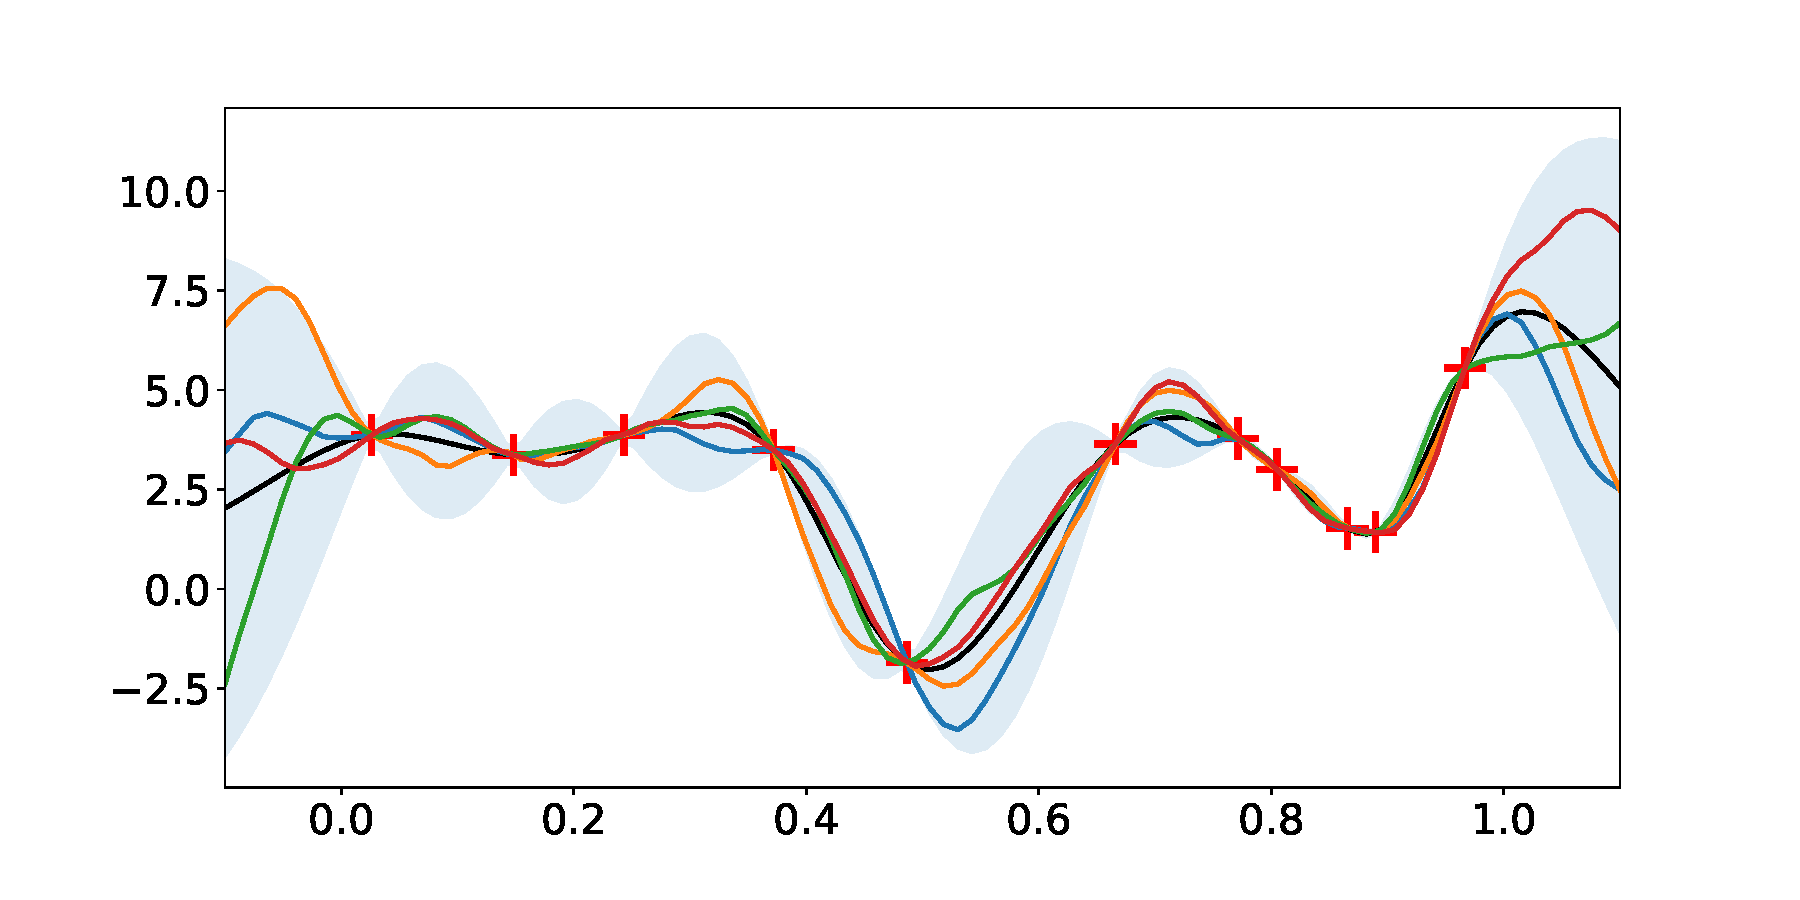
\includegraphics[trim=2.0cm 0.8cm 3.2cm 1.8cm, width=7.0cm]{figs/regression.pdf} }}
    \caption{A regression example: (a) Some observed data points, (b) Five samples of potential infinite number of functions that fit the observed data points.}%
    \label{FIG:1}
\end{figure}

\subsection{Gaussian Distribution}

A random variable $X$ is said to be Gaussian or normally distributed with mean $\mu$ and variance $\sigma^2$ if its probability density function (PDF) is \cite{Murphy2012}
\begin{ceqn}
    \begin{align}
       P_X(x) = \frac{1}{\sqrt{2 \pi} \sigma}\exp{\left(-\frac{{\left(x - \mu \right)}^{2}}{2 \sigma^{2}}\right)} \ . \nonumber
    \end{align}
\end{ceqn}
Here, $X$ represents random variables and $x$ is the real argument. The normal distribution of $X$ is usually represented by $ P(x) ~ \sim\mathcal{N}(\mu, \sigma^2)$. A one dimensional (1-d) Gaussian PDF was plotted in Fig. \ref{FIG:2}. We generated $n=1000$ numbers of random sample points from a 1-d Gaussian distribution and plotted them on the $x$ axis.
\begin{figure}[h!]
	\centering
		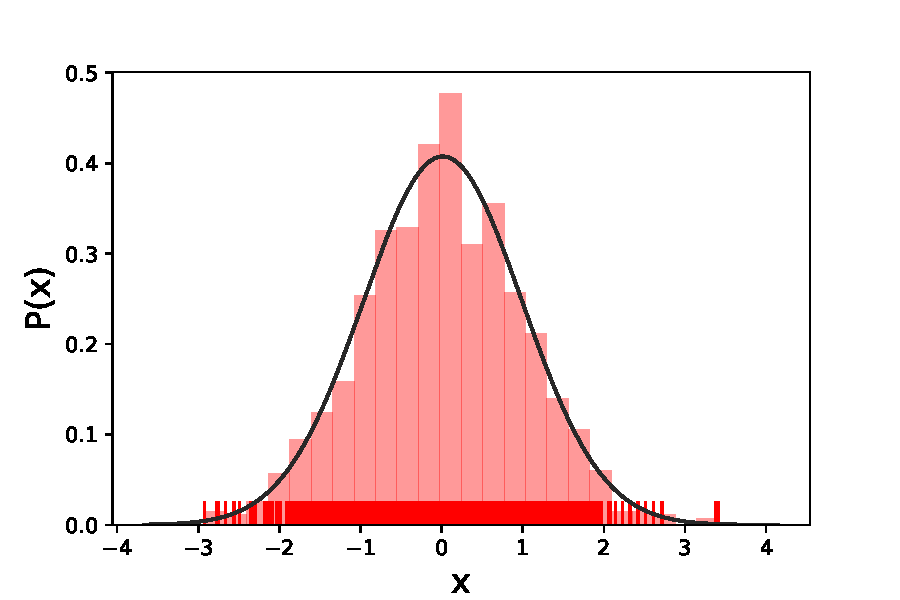
\includegraphics[trim=0.4cm 0.1cm 1.4cm 0.6cm, width=8.0cm]{figs/1d_random.pdf}
    	\caption{One thousand random sample points from a 1-d Gaussian was plotted as blue vertical bars on the $x$ axis. The PDF of these data points was plotted as a two dimensional bell curve.}
    	\label{FIG:2}
\end{figure}

These generated data can be viewed as a vector $X_1=[x^{(1)}, x^{(2)}, \ldots, x^{(n)}]$. By plotting the vector $X_1$ on a new $X$ axis at $X = 0$, we projected all points of $X_1$ to another space shown in Fig. \ref{FIG:3}. We did nothing but vertically plot points of the vector $X_1$ in the $X-f(X)$ coordinates space. We can plot another independent Gaussian vector $X_2$ within the same coordinates at $X = 1$. Keep in mind that each vector $X_1$ and $X_2$ is normal distributed shown in Fig. \ref{FIG:3}. Next, we random selected 10 point of $X_1$ and $X_2$ respectively and connected points of these 10 points in order by lines shown in Fig. \ref{FIG:4}(a). These lines look like linear functions spanning within the $[0, 1]$ domain.
\begin{figure}[h!]
	\centering
		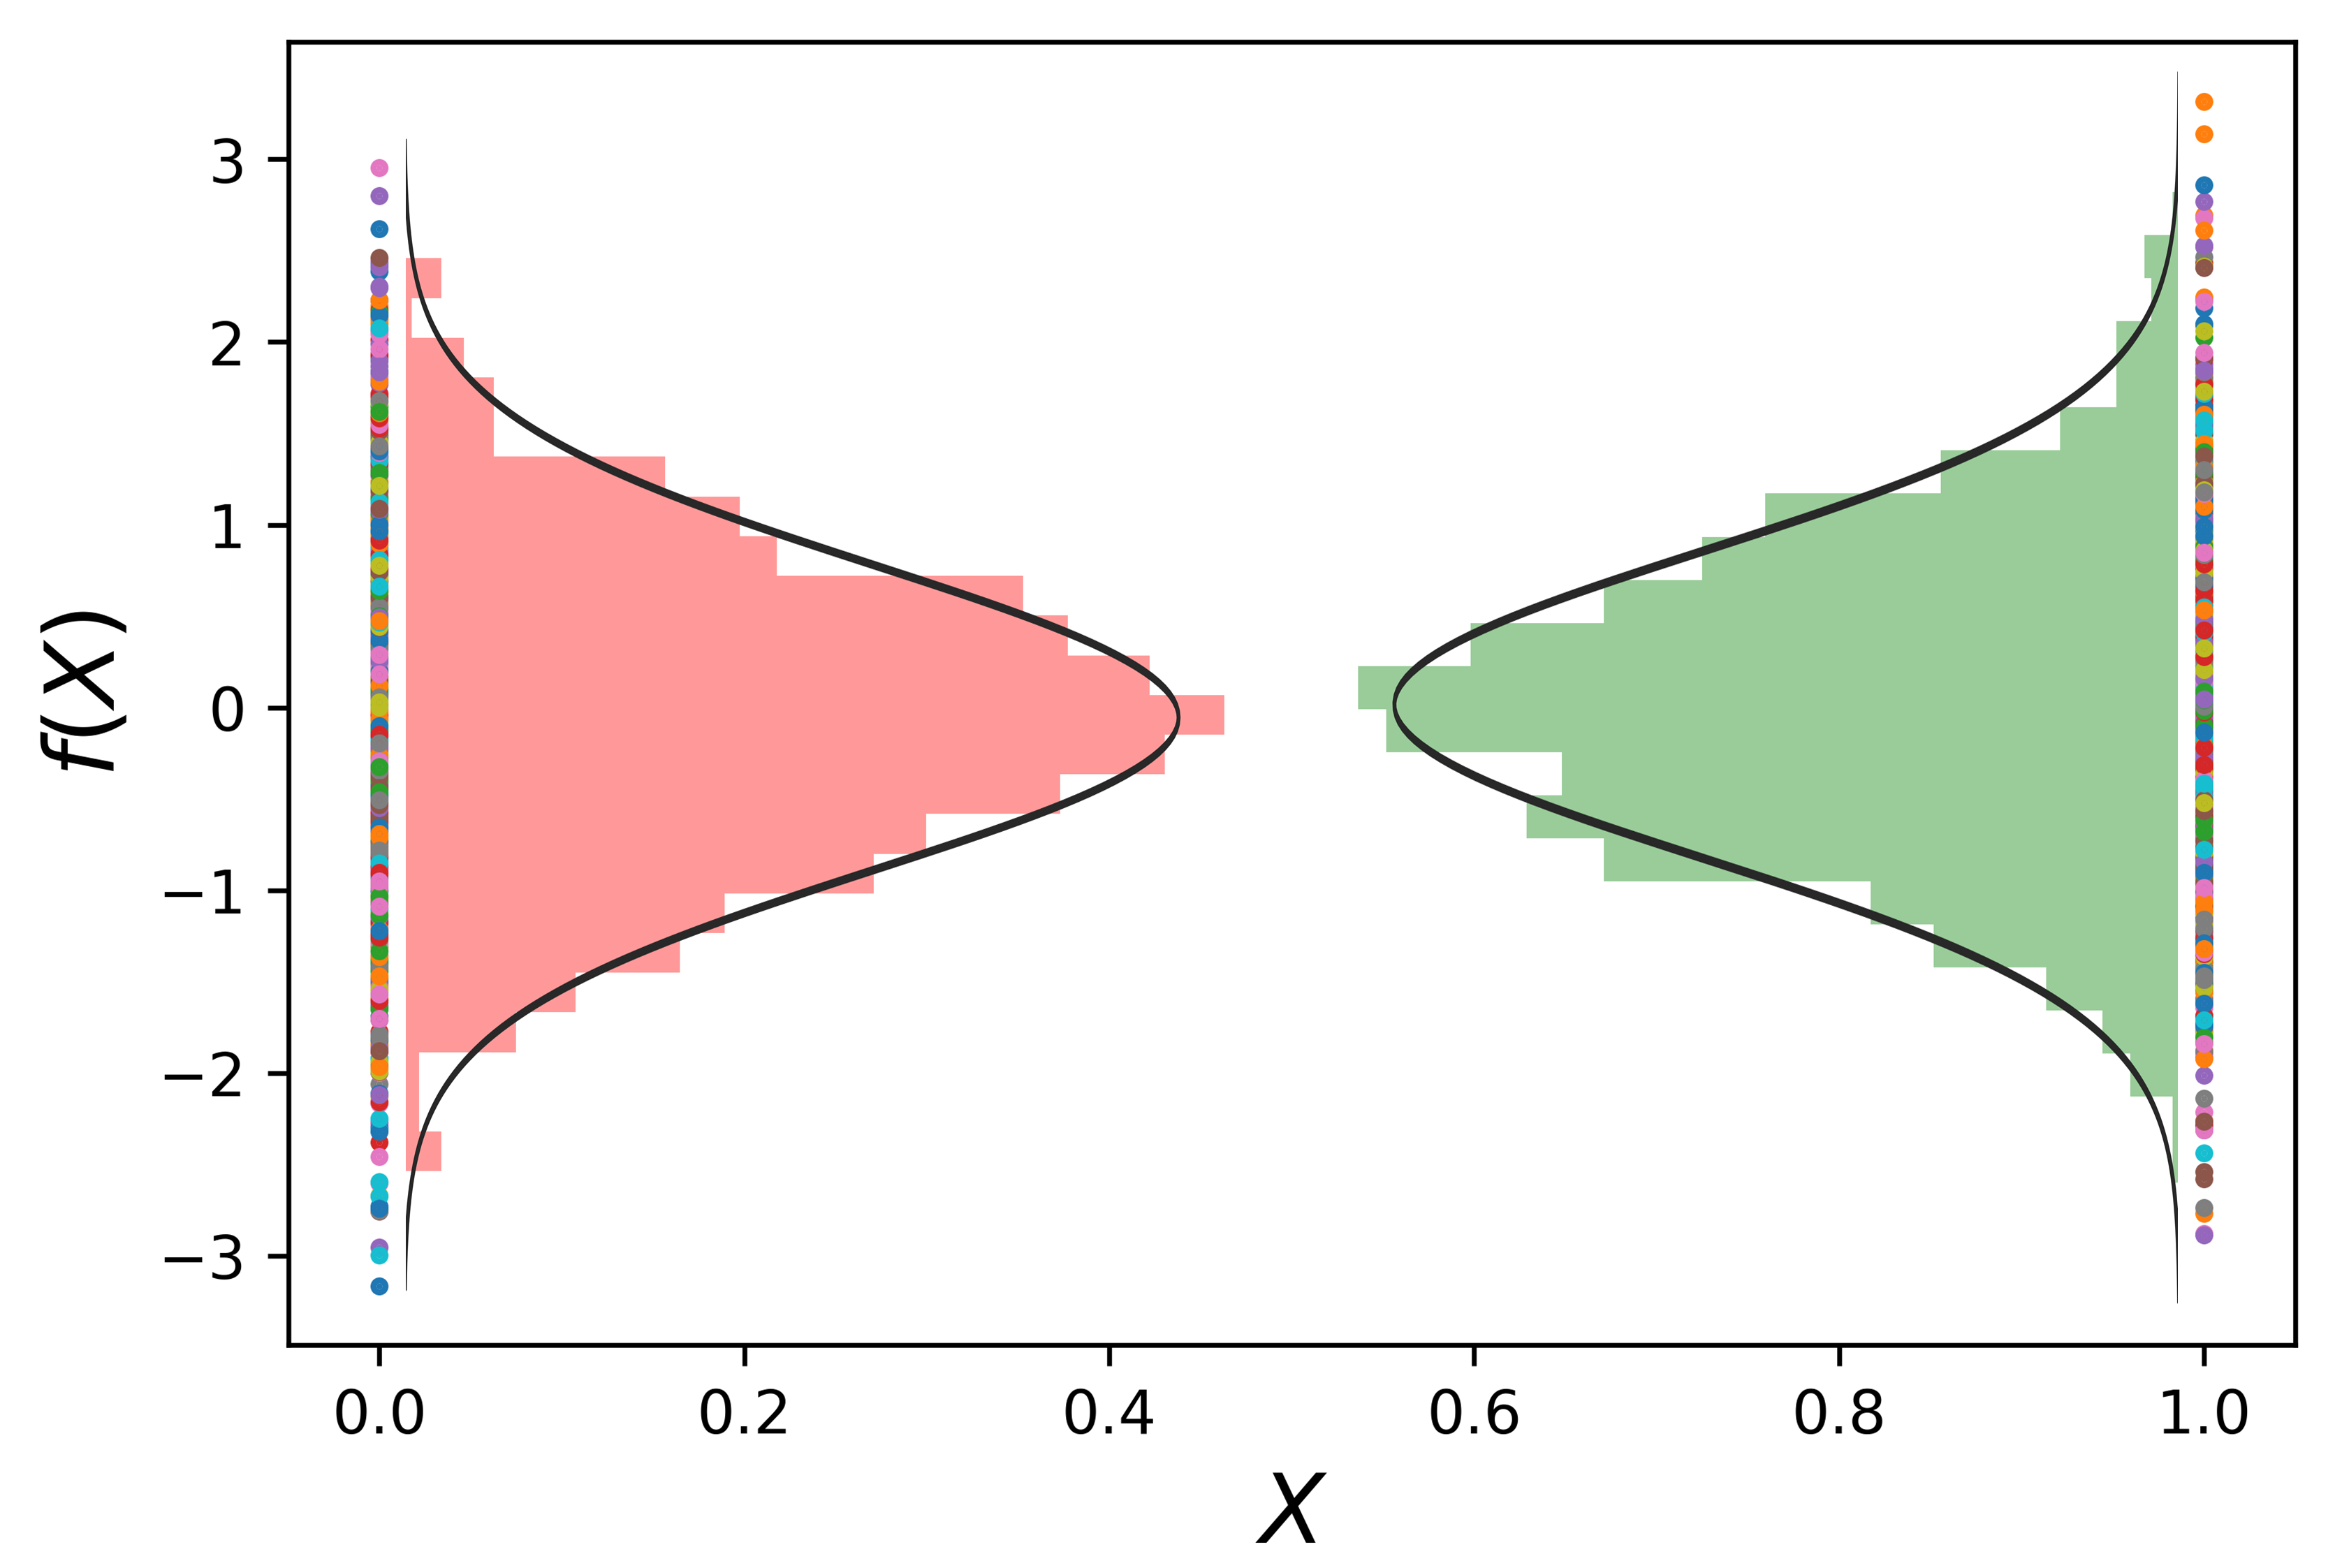
\includegraphics[width=11.0cm]{figs/2gaussian.png}
	\caption{Two independent 1-d Gaussian vector points were plotted vertically.}
	\label{FIG:3}
\end{figure}
Going back to think about regression, we can use these functions to make predictions if the new data points are on (or close enough to) these lines. The assumption that new data points are on the connected linear functions is too strong to be guaranteed because new data points can be anywhere within $[0, 1]$. If we plot more random generated normal distributed vectors, for example, 20 vectors $X_1, X_2, \ldots, X_{20}$ between $[0, 1]$, and connect 10 random selected sample points of each vector as lines shown in Fig. \ref{FIG:4}(b), we got 10 lines that look like functions within $[0, 1]$. However, we can't use these lines to make predictions for regression tasks because they are too noisy. These functions must be smoother, meaning input points that are close to each other should have similar output function values. In a word, ``functions'' by connecting random generated independent Gaussian points are not smooth enough for regression tasks, we need these independent Gaussian distributions correlated to each other as joint Gaussian distributions. The joint Gaussian distribution is described by the multi-variable Gaussian theory.  
\begin{figure}[h!]
    \centering
    \subfloat[Two Gaussian vectors]{{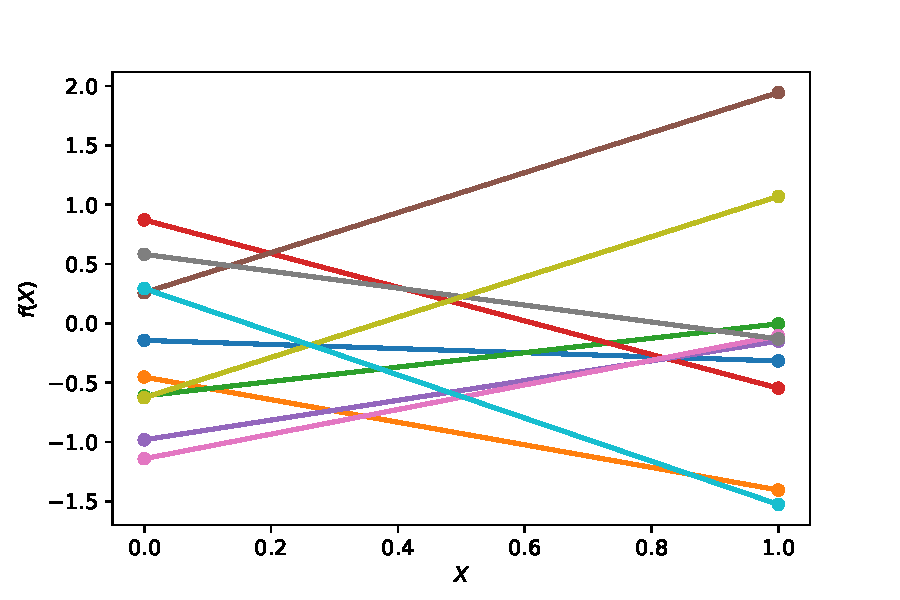
\includegraphics[trim=0.3cm 0.3cm 1.6cm 1.1cm, width=7.05cm]{figs/random_x1_x2.pdf} }}
    \qquad
    \subfloat[Twenty Gaussian vectors]{{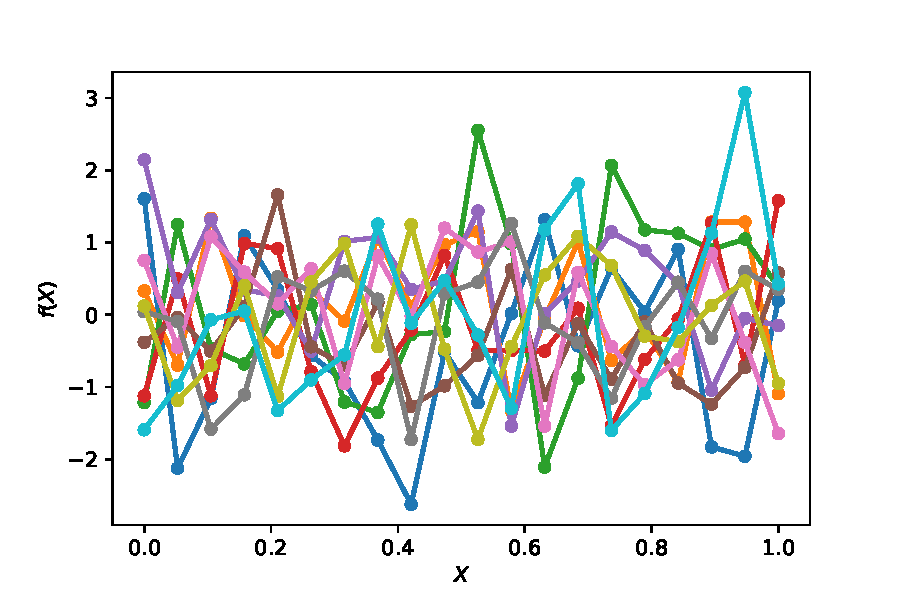
\includegraphics[trim=0.6cm 0.3cm 1.6cm 1.1cm, width=6.95cm]{figs/random_x1_x20.pdf} }}
    \caption{Connecting points of independent Gaussian vectors by lines.}%
    \label{FIG:4}
\end{figure}

\subsection{Multivariate Normal Distribution}

In many situations, a system (set of data) is described by more than one feature variables $[X_1, X_2, \ldots, X_D]$ that are correlated to each other. If we want to model the variables all together as one Gaussian model, it's a multivariate Gaussian/normal (MVN) \cite{Murphy2012} distribution model. We use a two dimensional (2-d) MVN model as an example. A 2-d MVN can be visualized as a three dimensional (3-d) bell curve with height represents the probability density shown in Fig. \ref{FIG:5}a. The 3-d bell curve projection on the $x_1-x_2$ plane plotted in Fig. \ref{FIG:5}a and \ref{FIG:5}b are ellipse contours showing the co-relationship between $x_1$and $x_2$ points. The $P(x_1, x_2)$ is the joint probability of $X_1$ and $X_2$. 
\begin{figure}[h!]
    \centering
    \subfloat[3-d bell curve]{{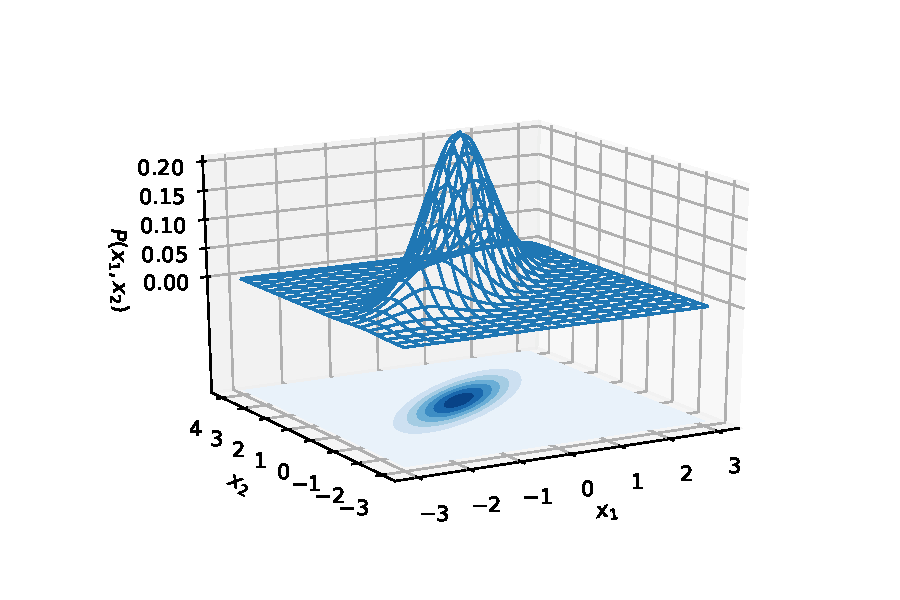
\includegraphics[trim=1.6cm 1.0cm 2.6cm 1.0cm, width=8.6cm]{figs/3d_gaussian_example.pdf} }}
    \qquad
    \subfloat[2-d ellipse contours]{{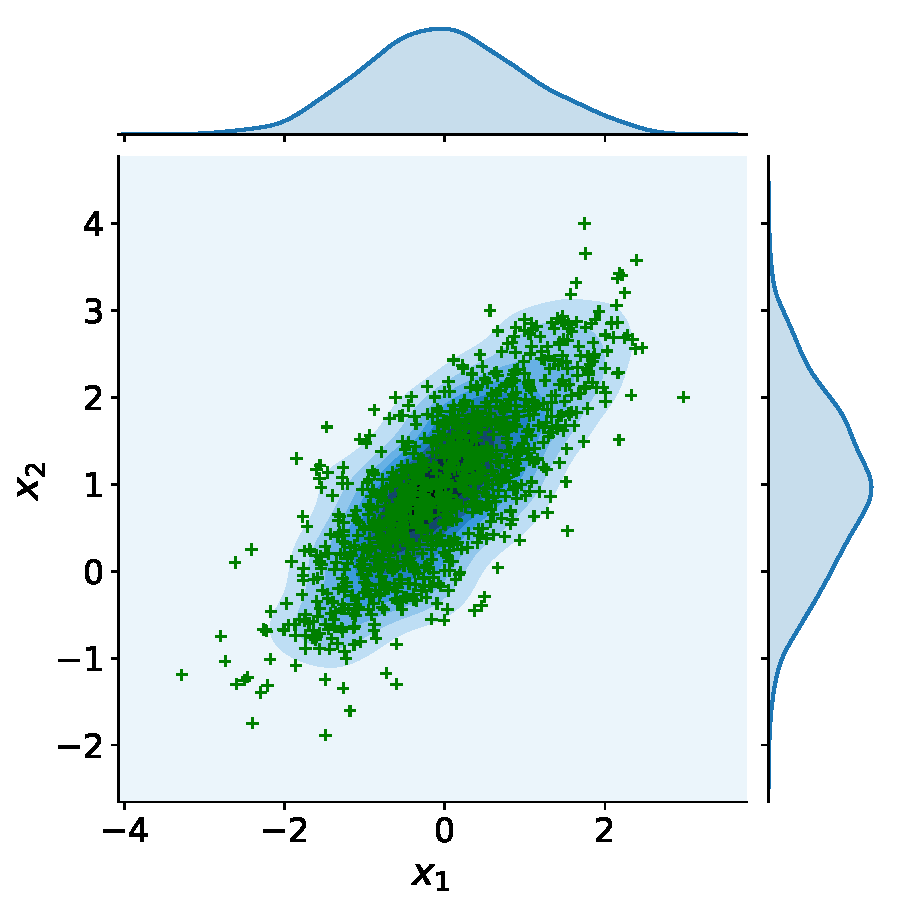
\includegraphics[trim=0.3cm 0.0cm 0.8cm 0.6cm, width=5.5cm]{figs/2d_gaussian_example.pdf} }}
    \caption{The PDF of a 2-d MVN visualization: (a) a 3-d bell curve with height represents the probability density, (b) ellipse contour projections showing the co-relationship between $x_1$and $x_2$ points.}%
    \label{FIG:5}
\end{figure}

Formally, the PDF of the MVN with D dimension is defined as \cite{Murphy2012}
\begin{ceqn}
    \begin{align}
       \mathcal{N}(x | \mu,\Sigma) = \dfrac{1}{(2\pi)^{D/2}|\Sigma|^{1/2}}\exp\left[-\dfrac{1}{2}(x-\mu)^\mathsf{T} \Sigma^{-1}(x-\mu)\right] \ , \nonumber
    \end{align}
\end{ceqn}
where $D$ is the number of dimension, $x$ represents the variable, $\mu=\mathbb{E}[x] \in \mathbb{R}^D$ is the mean vector, and $\Sigma=\operatorname{cov}[x]$ is the $D \times D$ covariance matrix. The $\Sigma$ is a symmetric matrix that stores the pairwise covariance of all the jointly modeled random variables with its $(i,j)$ element as $\Sigma_{ij}=\operatorname{cov}(y_i,y_j)$. For a 2-d MVN, the mean vector $\mu$ is a 2-d vector $\begin{bmatrix} \mu_1 \\ \mu_2 \end{bmatrix}$, which are independent mean of each variable $x_1$ and $x_2$. The covariance matrix is $\begin{bmatrix} \sigma^2_1 & \sigma_{12} \\ \sigma_{21} & \sigma^2_2 \end{bmatrix}$. The diagonal terms are independent variance of each variable $x_1$ and $x_2$. The off-diagonal terms represents correlations between the two variables that represents how much one variable $x_1$ is related to another variable $x_2$. A 2-d Gaussian is expressed as 
\begin{ceqn}
    \begin{align}
       \begin{bmatrix} x_1 \\ x_2 \end{bmatrix} \sim \mathcal{N}\left(\begin{bmatrix} \mu_1 \\ \mu_2 \end{bmatrix}, \begin{bmatrix} \sigma^2_1 & \sigma_{12} \\ \sigma_{21} & \sigma^2_2 \end{bmatrix}\right) \sim \mathcal{N}(\mu, \Sigma) \ . \nonumber
    \end{align}
\end{ceqn}
Instead of the joint probability, we are more interested to the conditional probability for the regression tasks. If we cut a slice on the 3-d bell curve or draw a line on the ellipse contours shown in Fig. \ref{FIG:5}, we get the conditional probability distribution $P(x_1 \vert \, x_2)$ shown in Fig. \ref{FIG:6}. The conditional distribution is also Gaussian \cite{Rasmussen2006}.
\begin{figure}[h!]
	\centering
		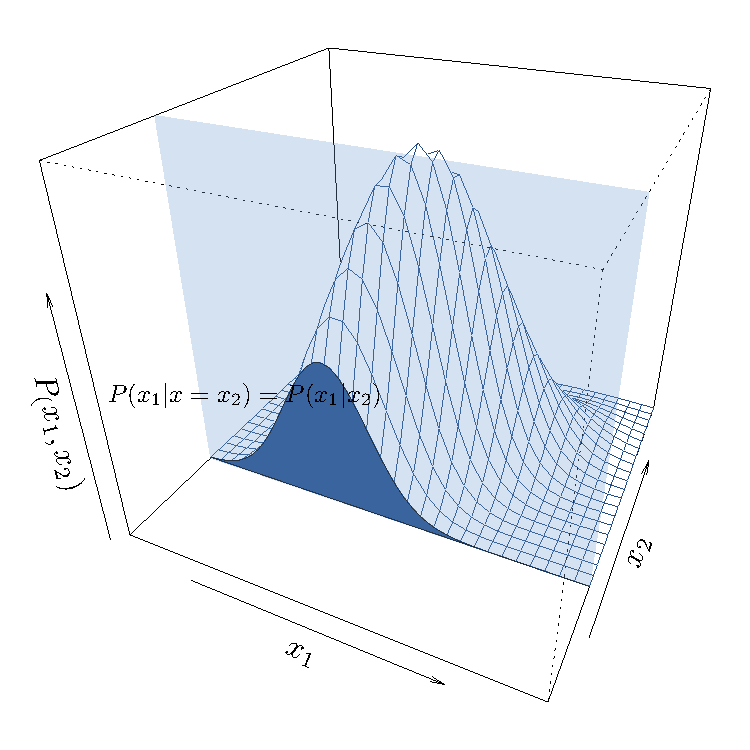
\includegraphics[trim=0.4cm 0.4cm 0.6cm 0.8cm, width=10.0cm]{figs/2d_gaussian_conditional.pdf}
	\caption{The conditional probability distribution $P(x_1 \vert \, x_2)$.}
	\label{FIG:6}
\end{figure}

\subsection{Kernels}

After reviewing MVN, we smooth the functions in Fig. \ref{FIG:4}(b) by defining the covariance functions. For regression tasks, outputs of the function should be similar when two input points are similar to each other. One possible function format is dot product function due to the fact that when two input vectors are similar, their dot product output value is high. It is clear in the dot product equation $A \cdot B = \lVert A \rVert \lVert B \rVert \operatorname{cos}\theta$, where $\theta$ is the angle between two input vectors. In fact, if a function is defined solely in terms of inner products in input space as $k(x,\ x^\prime)$; we call $k(\cdot, \cdot)$ a kernel function \cite{Rasmussen2006}. The most widely used covariance function (kernel function) is the squared exponential kernel function. It's also called the radial basis function (RBF) kernel or Gaussian kernel function that is defined as \footnote{This is a simplified RBF without hyperparameters for simplicity. A general RBF is explained in section \ref{Hyperparameters}.} 
\begin{ceqn}
    \begin{align}
       \operatorname{cov}(x_i, x_j)=\exp\left(-~\frac{(x_i-x_j)^2}{2}\right) \ . \nonumber
    \end{align}
\end{ceqn}

Let's re-plot 20 independent Gaussian vector points and connecting points in order by lines shown in Fig. \ref{FIG:4}(b). Instead of 20 independent Gaussian that has 10 sample points in each vector, we generated 10 twenty dimensional (20-d) MVN with an identity covariance matrix function shown in \ref{FIG:7}(a). It's the same as \ref{FIG:4}(b) because there is no smoothness added by using an identity covariance matrix as its kernel function. When the RBF was used as the covariance function to generate 10 samples of 20-d MVN, we got smooth lines shown in \ref{FIG:7}(b).
\begin{figure}[h!]
    \centering
    \subfloat[10 samples of the 20-d MVN prior with identity kernel]{{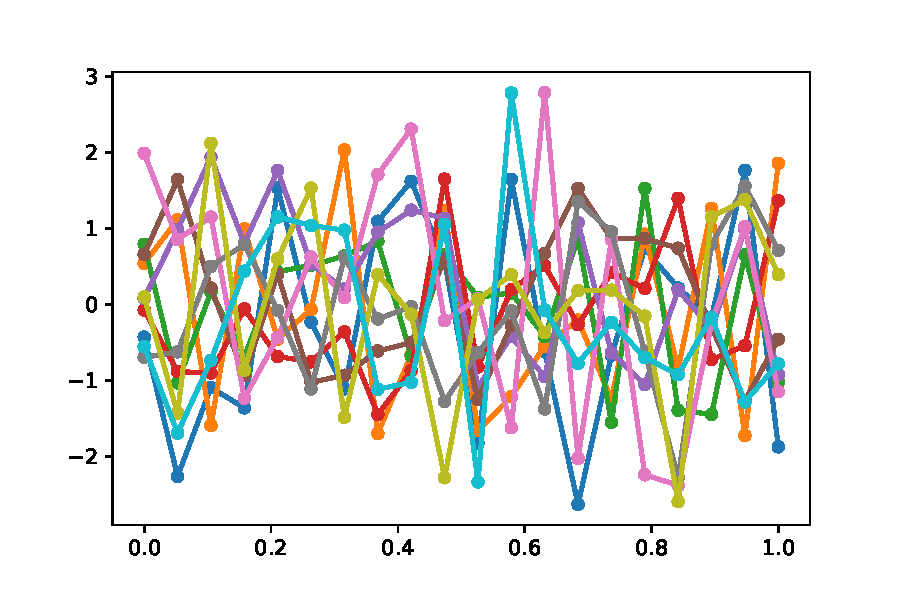
\includegraphics[trim=1.2cm 0.4cm 1.6cm 1.1cm, width=6.9cm]{figs/20d_gaussian_prior.pdf} }}
    \qquad
    \subfloat[10 samples of the 20-d MVN prior with RBF kernel]{{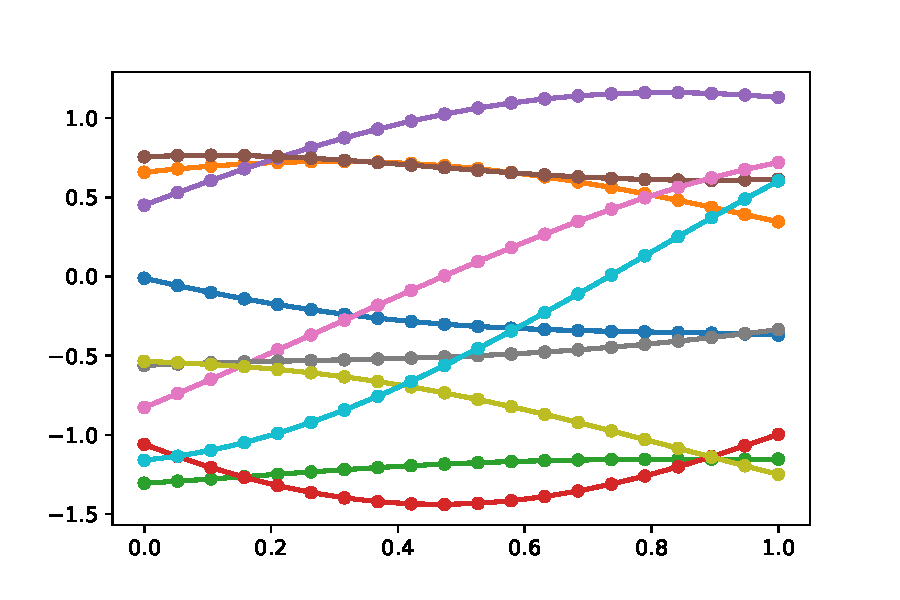
\includegraphics[trim=0.9cm 0.4cm 1.6cm 1.1cm, width=7.1cm]{figs/20d_gaussian_kernel_prior.pdf} }}
    \caption{Ten samples of 20-d MVN kernelized prior functions.}%
    \label{FIG:7}
\end{figure}

We get smooth lines and they look more like functions. It's natural to consider to continue increasing the dimension of MVN. When the dimension of MVN gets larger, the region of interest is filled up with more points. When the dimension becomes infinity, there is a point that represents any possible input. By using infinity dimensional MVN, we are fitting functions with infinity parameters for regression tasks. We can make predictions anywhere in the region of interest. We can plot `m=200' samples of a `n=200' dimensional MVN to get a feeling of functions with infinity parameters shown in Fig. \ref{FIG:8}. We call these functions as kernelized prior functions because there are no observed data points yet. All functions are generated by the MVN model incorporating kernel function as prior knowledge before having any observed data points. 
\begin{figure}[h!]
	\centering
		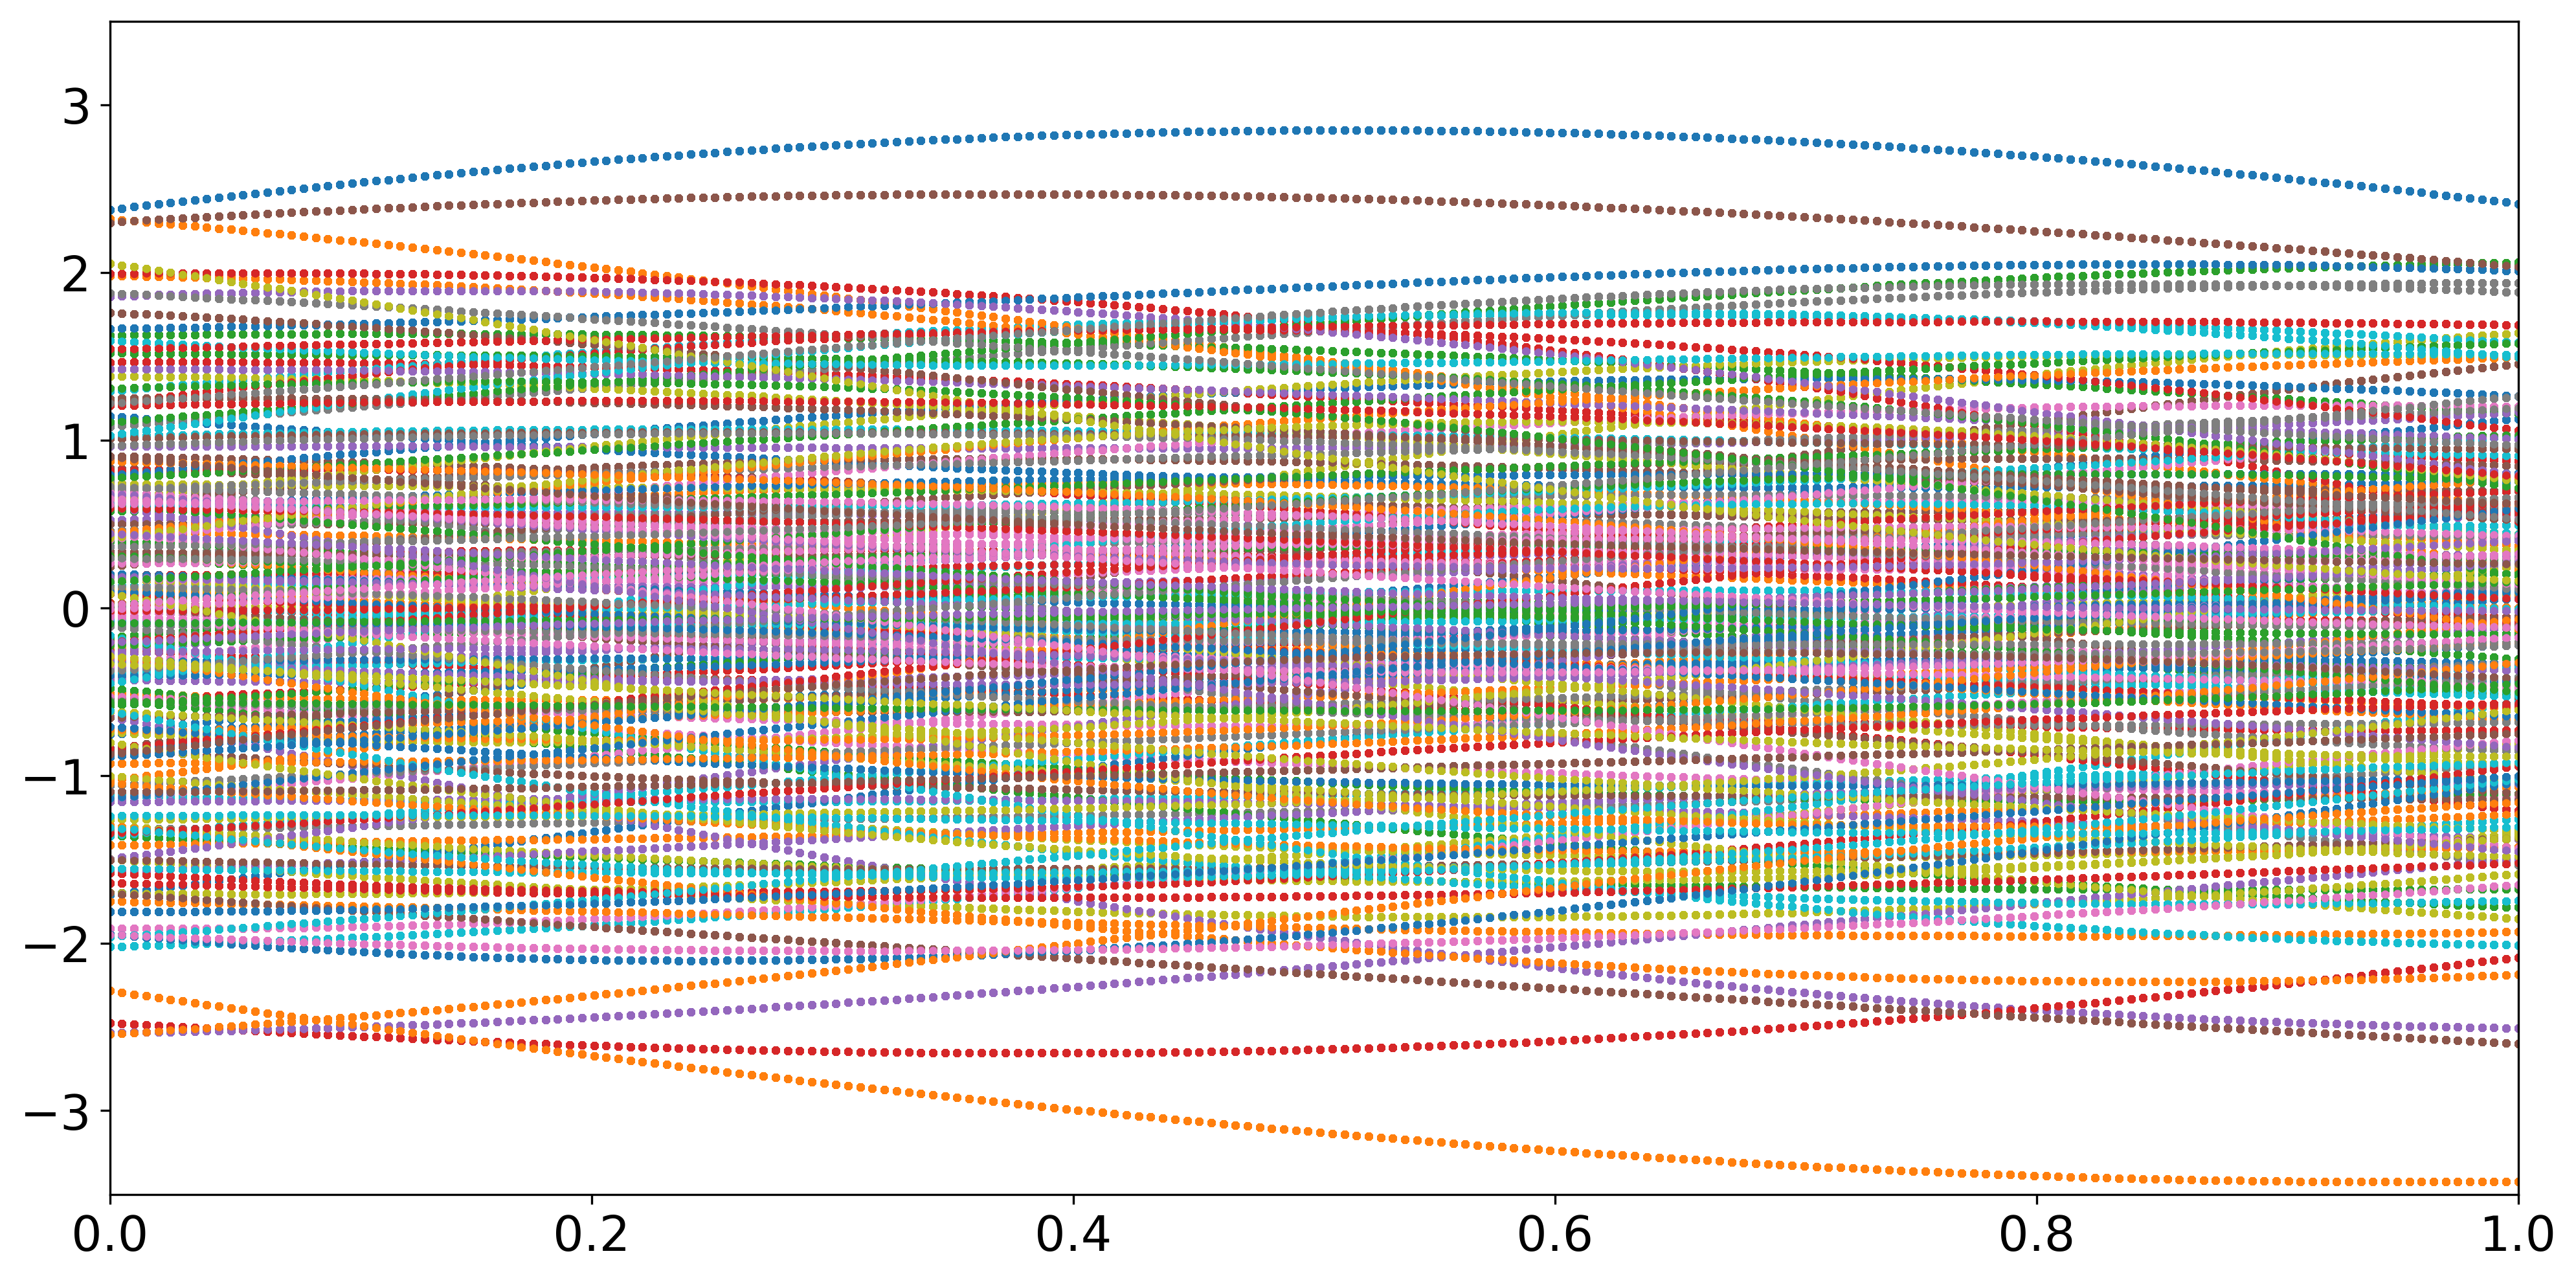
\includegraphics[width=13.0cm]{figs/200d_gaussian_kernel_prior.png}
	\caption{200 samples of a 200 dimensional MVN kernelized prior functions.}
	\label{FIG:8}
\end{figure}

\subsection{Nonparametric model}

This section explains the basics of parametric and nonparametric models \cite{Murphy2012}. Parametric models assume that the data distribution can be modeled in terms of a set of finite numbers of parameters. In regression, given some data points, we would like to make predictions of the function value $y=f(x)$ with a specific $x$. If we assume a linear regression model, $y = \theta_1  + \theta_2 x$, we need to find the parameters $\theta_1$ and $\theta_2$ to define the function. In many cases, the linear model assumption isn’t hold, a polynomial model with more parameters, such as $y = \theta_1+\theta_2 x+\theta_3 x^2$ is needed. We use the training dataset $D$ with $n$ observed points, $D=[(x_i,y_i)\, \vert \, i=1,…,n]$ to train the model, i.e. mapping $x$ to $y$ through parameters $ \boldsymbol {\theta}= (\theta_1,\theta_2,\theta_3)$. After the training process, we assume all the information of the data is captured by the feature parameters $\boldsymbol {\theta}$, thus predictions are independent of the training dataset $D$. It can be expressed as  $P(f_* \, \vert \,  X_*, \boldsymbol {\theta} ,D)=P(f_* \, \, \vert \,  X_*, \boldsymbol {\theta})$, in which $f_*$ are predictions made at unobserved data points $X_*$. Thus, conducting regression using parametric models, the complexity or flexibility of the model is limited by the parameter numbers. It’s natural to think to use a model that the number of parameters grows with the size of the dataset, and it’s a Bayesian nonparametric model. The Bayesian nonparametric model doesn't imply that there are no parameters, but rather infinite parameters. 

\section{Math}

\subsection{Definition}
Before diving into equations, let's review the covered mathematical basics. In regression, there is a function $\mathbf{f}$ we are trying to model given a set of data points $\mathbf{X}$ (training data/existing observed data) from the unknown function $\mathbf{f}$. The traditional nonlinear regression methods typically give one function that is considered to fit the dataset best. However, there may be more than one function that can fit the observed data points equally well. We saw that when the dimension of MVN is infinite, we can make predictions at any point with these infinite number of functions. These functions are MVN because it's our assumption (prior). More formally, the prior distribution of these infinite functions is MVN. The prior distribution representing the outputs $\mathbf{f}$ that we expect to see over some inputs $\mathbf{x}$ without observing any data. When we start to have observation points, instead of infinite functions, we keep functions that fit the observed points. Now we got the posterior, the current belief based on existing observations. When we have new observation points, we use the current posterior as the prior, use new observation points to update the posterior.  

This is \textbf{Gaussian processes}: A Gaussian processes model is a probability distribution over possible functions that fit a set of points. Because we have the probability distribution over all possible functions, we can calculate the means as the function, and the variances to indicate how confident the predictions are. The key points are summarized as 1) the functions(posterior) updates with new observations. 2) The mean function calculated by the posterior distribution of the possible infinity functions is the function used for regression predictions. 3) A Gaussian processes model is a probability distribution over possible functions, and any finite sample of functions is jointly Gaussian distributed.

\subsection{Predictions}
This section provides a concise description of the standard Gaussian processes algorithm. The parameter definition follows \cite{Rasmussen2006}. Besides the covered mathematics foundation, it's highly recommended to read Appendix A.1 and A.2 of \cite{Rasmussen2006} before continuing to read. The regression function is modeled by a multivariate Gaussian as 
\begin{ceqn}
    \begin{align}
       P(\mathbf{f} \, \lvert\, \mathbf{X}) = \mathcal{N}(\mathbf{f} \, \lvert\, \boldsymbol\mu, \mathbf{K}) \ , \nonumber
    \end{align}
\end{ceqn}
where $\mathbf{X} = [{x}_1,...,{x}_n ]$, $\mathbf{f} = \left[ f(\mathbf{x}_1),...,f(\mathbf{x}_n) \right]$, $\boldsymbol\mu = \left[ m(\mathbf{x}_1),...,m(\mathbf{x}_n) \right]$ and $K_{ij} = k(\mathbf{x}_i,\mathbf{x}_j)$. $\mathbf{X}$ is the observed data points, $m$ represents the mean function and it is common to set $m(\mathbf{x}) = 0$ as Gaussian processes is flexible enough to model the mean arbitrarily well. $k$ represents a positive definite kernel function. The Gaussian processes model is a distribution over functions whose shape (smoothness) is defined by $\mathbf{K}$. If points $\mathbf{x}_i$ and $\mathbf{x}_j$ are considered to be similar by the kernel, the function output values at the two points, $f(\mathbf{x}_i)$ and $f(\mathbf{x}_j)$, are expected to be similar. The regression by Gaussian processes is illustrated in Fig. \ref{FIG:9}: given some observed data points (red points) and a mean function $\mathbf{f}$ estimated by these points (blue line), we make predictions at some new points $\mathbf{X}_*$ as $f(\mathbf{X}_*)$.
\begin{figure}[h!]
	\centering
		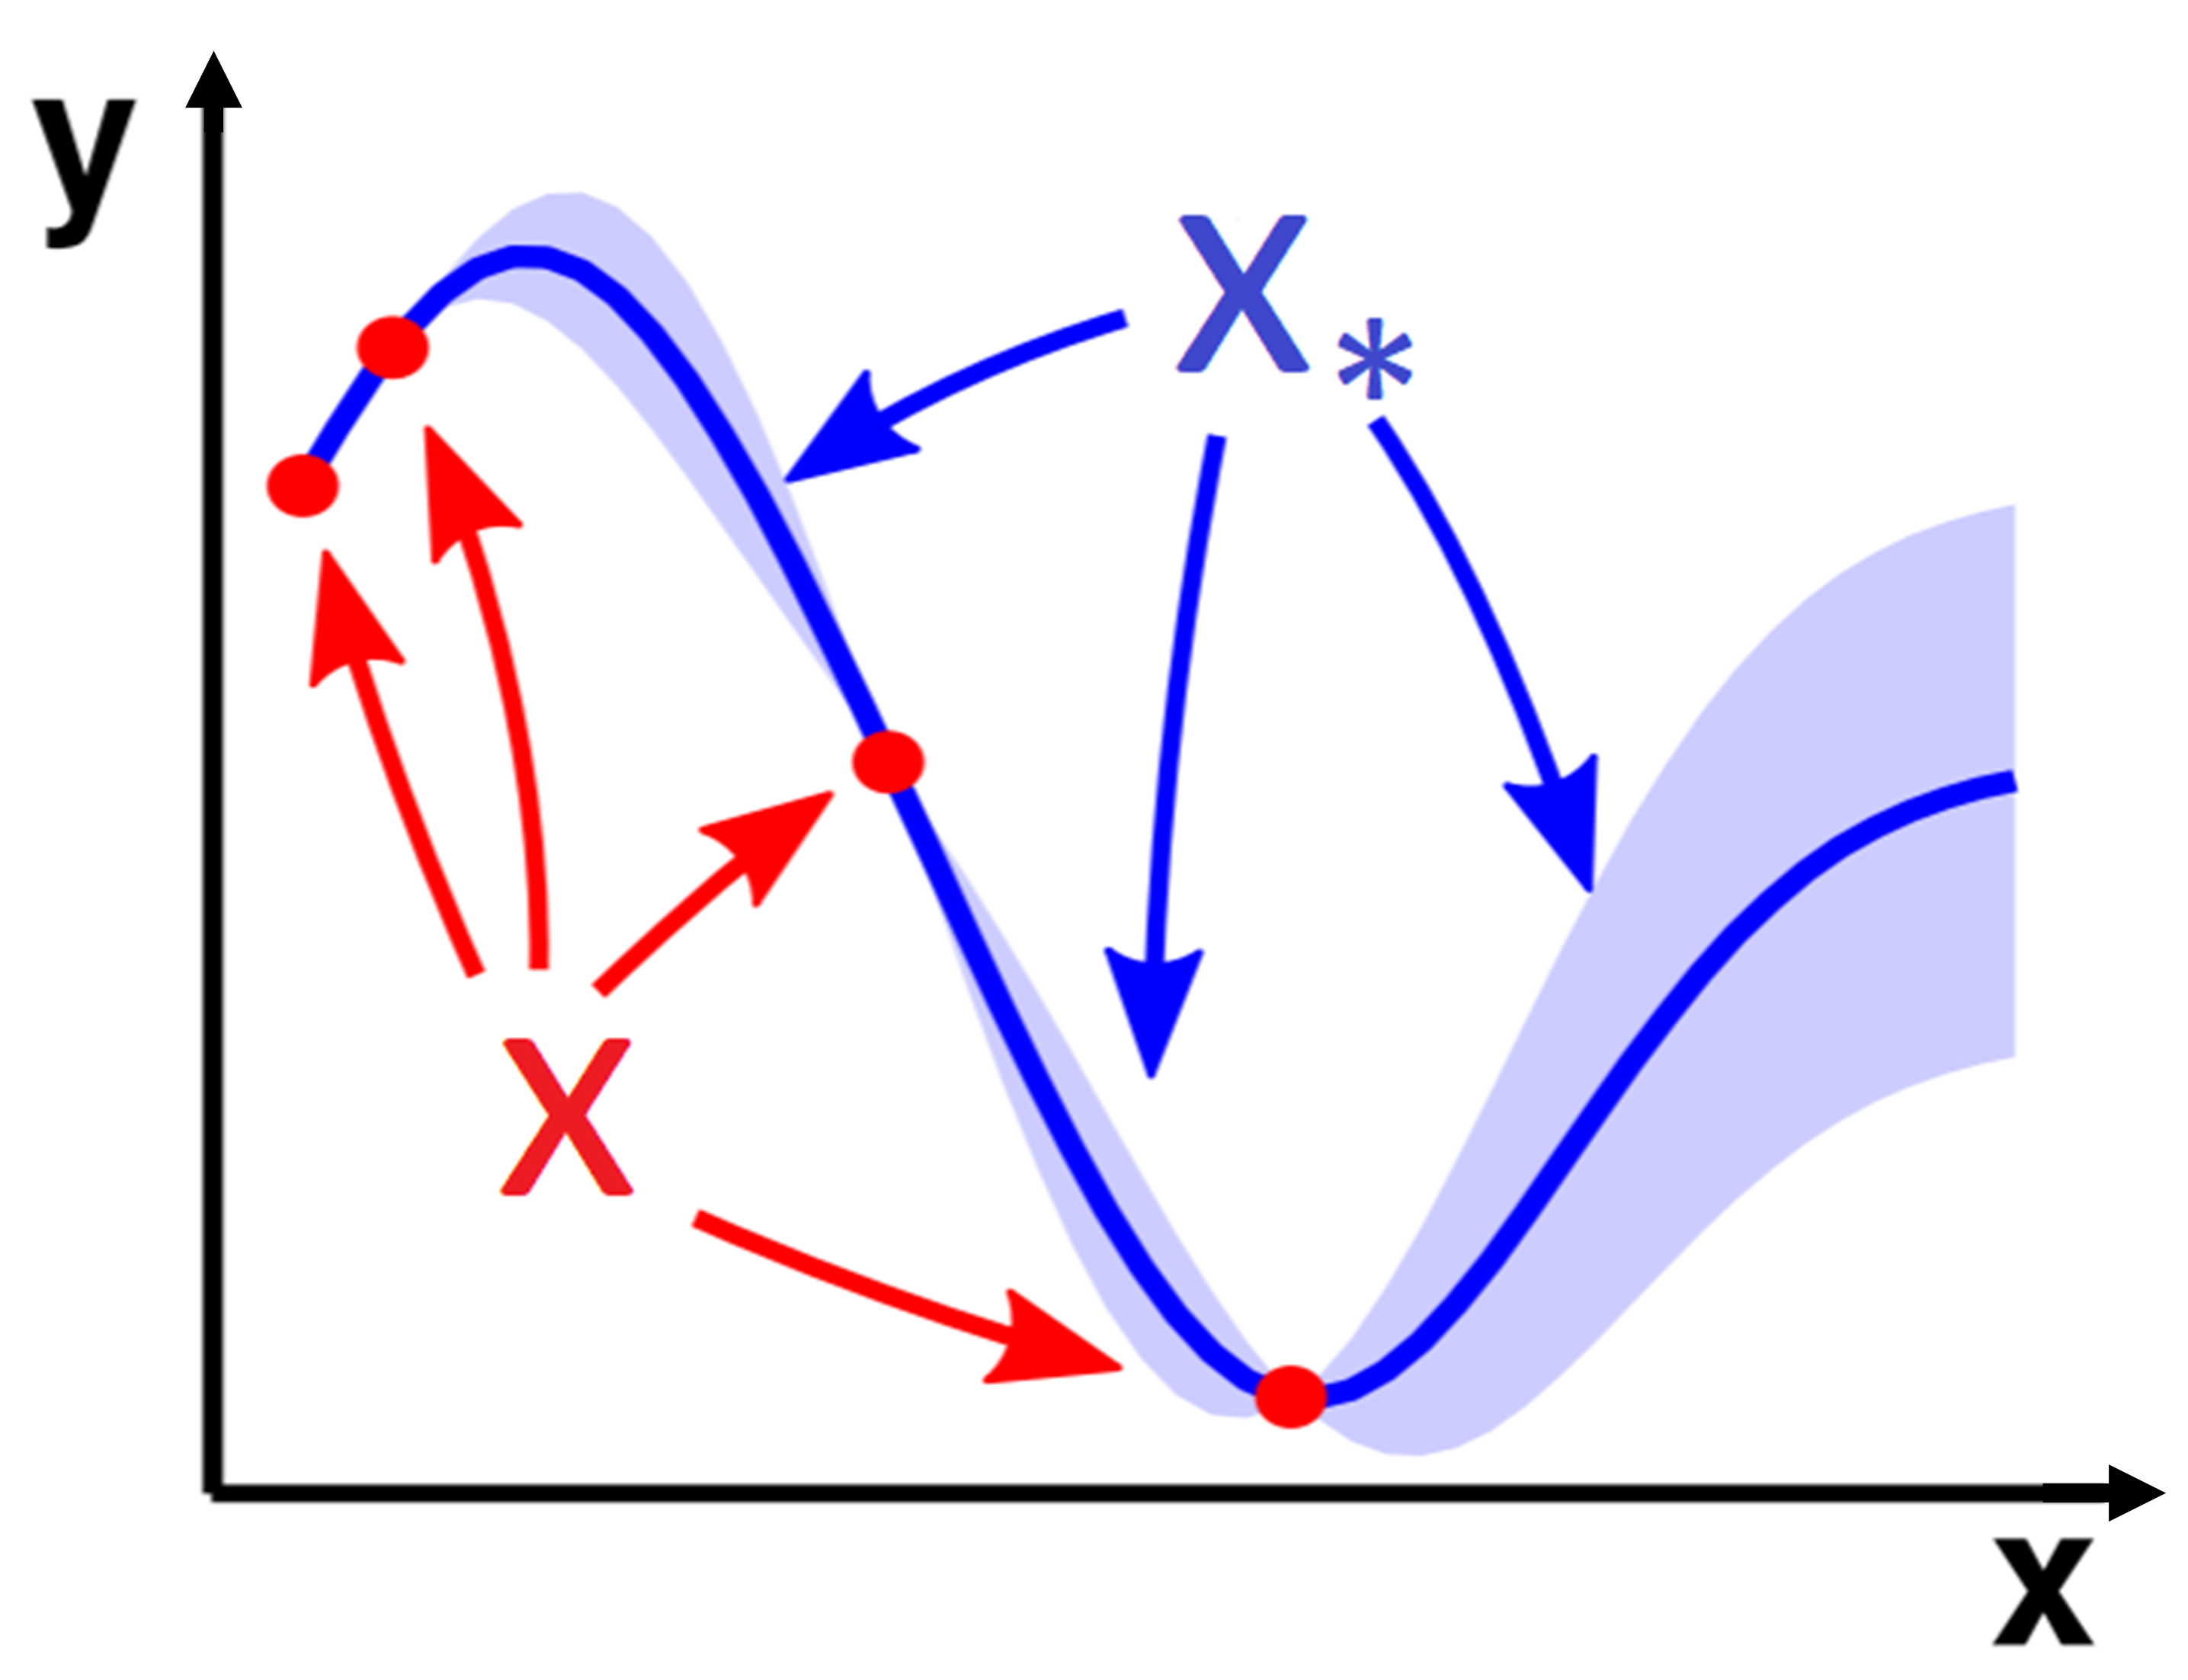
\includegraphics[scale=.25]{figs/predictions.png}
	\caption{The illustrative process of Gaussian processes regression.}
	\label{FIG:9}
\end{figure}

The joint distribution of $\mathbf{f}$ and $\mathbf{f}_*$ is expressed as
\begin{ceqn}
    \begin{align}
       \begin{bmatrix}\mathbf{f} \\ \mathbf{f}_*\end{bmatrix} \sim \mathcal{N}\left(\begin{bmatrix}m(\mathbf{X})\\ m(\mathbf{X}_*)\end{bmatrix}, \begin{bmatrix}\mathbf{K} & \mathbf{K}_* \\ \mathbf{K}_*^\mathsf{T} & \mathbf{K}_{**}\end{bmatrix}\right) \ , \nonumber
    \end{align}
\end{ceqn}
where $\mathbf{K}=K(\mathbf{X}, \mathbf{X})$, $\mathbf{K}_* = K(\mathbf{X}, \mathbf{X}_*)$ and $\mathbf{K}_{**}=K(\mathbf{X}_*, \mathbf{X}_*)$. And $\begin{pmatrix}m(\mathbf{X}), m(\mathbf{X}_*)\end{pmatrix} = \mathbf{0}$. 

This is the joint probability distribution equation $P(\mathbf{f}, \mathbf{f}_* \, \vert \, \mathbf{X}, \mathbf{X}_*)$ over $\mathbf{f}$ and $\mathbf{f}_*$, but regression tasks need the conditional distribution $P(\mathbf{f}_* \, \vert \, \mathbf{f}, \mathbf{X}, \mathbf{X}_*)$ over $\mathbf{f}_*$ only. The derivation from the joint distribution $P(\mathbf{f}, \mathbf{f}_* \, \vert \, \mathbf{X}, \mathbf{X}_*)$ to the conditional $P(\mathbf{f}_* \, \vert \, \mathbf{f}, \mathbf{X}, \mathbf{X}_*)$ uses the theorem in Appendix \ref{APPENDIX}. The result is
\begin{ceqn}
    \begin{align}
       \mathbf{f}_* \, \vert \, \mathbf{f}, \mathbf{X}, \mathbf{X}_* \sim \mathcal{N} \left(\mathbf{K}_*^\mathsf{T} \, \mathbf{K} \, \mathbf{f}, \: \mathbf{K}_{**} - \mathbf{K}_*^\mathsf{T} \, \mathbf{K}^{-1} \, \mathbf{K}_* \right) \ . \nonumber
    \end{align}
\end{ceqn}
In more realistic situations, we don't have access to true function values but noisy versions thereof $y = f(x) + \epsilon$. Assuming there is an additive independent and identically distributed (i.i.d.) Gaussian noise with variance $\sigma_n^2$, the prior on the noisy observations becomes $\operatorname{cov}(y) = \mathbf{K} + \sigma_n^2 {I}$. The joint distribution of the observed values and the function values at the new testing points becomes
\begin{ceqn}
    \begin{align}
       \begin{pmatrix}\mathbf{y} \\ \mathbf{f}_*\end{pmatrix} \sim\mathcal{N}\left(\mathbf{0}, \begin{bmatrix}\mathbf{K} + \sigma_n^2 {I} & \mathbf{K}_* \\ \mathbf{K}_*^\mathsf{T} & \mathbf{K}_{**}\end{bmatrix}\right) \ . \nonumber
    \end{align}
\end{ceqn}
By deriving the conditional distribution, we get the predictive equations for Gaussian processes regression as
\begin{ceqn}
    \begin{align}
       \mathbf{\bar{f}_*} \, \vert \, \mathbf{X}, \mathbf{y}, \mathbf{X}_* \sim \mathcal{N} \left(\mathbf{\bar{f}_*}, \operatorname{cov}(\mathbf{f}_*)\right) \ , \nonumber
    \end{align}
\end{ceqn}
where 
\begin{ceqn}
    \begin{align}
        \mathbf{\bar{f}_*} &\overset{\Delta}{=} \mathbb{E} [\mathbf{\bar{f}_*} \, \vert \, \mathbf{X}, \mathbf{y}, \mathbf{X}_*] = \mathbf{K}_*^\mathsf{T} [\mathbf{K} + \sigma_n^2{I}]^{-1} \mathbf{y} \ , \nonumber \\
        \operatorname{cov}(\mathbf{f}_*) &= \mathbf{K}_{**} - \mathbf{K}_*^\mathsf{T} [\mathbf{K} + \sigma_n^2{I}]^{-1} \mathbf{K}_* \ . \nonumber
    \end{align}
\end{ceqn}
It's clear from above equations that the training data are explicitly used for the new test data to construct the prediction distribution \cite{snelson2006sparse}, thus also proves that GP is a nonparametric model. 
\section{Illustrative example}

In this section, a example implementation of the Gaussian processes regression is shown. The implementation follows the algorithm in \cite{Rasmussen2006} as follows. 
\begin{ceqn}
    \begin{equation}\label{eqn:Marginals-and-conditionals-of-an-MVN}
      \boxed{\begin{split}
        L &= \operatorname{cholesky}(K + \sigma^2_n I) \\
        \boldsymbol{\alpha} &= L^{\top} \setminus (L \setminus \mathbf{y}) \\
    	\bar{f_{*}} &= \mathbf{k}_{*}^{\top} \boldsymbol{\alpha} \\
    	\mathbf{v} &= L \setminus \mathbf{k}_{*} \\
    	\mathbb{V}[f_{*}] &= k(\mathbf{x}_{*}, \mathbf{x}_{*}) - \mathbf{v}^{\top} \mathbf{v}.\\ 
    	\log p(\mathbf{y} \mid X) &= -\frac{1}{2} \mathbf{y}^{\top} (K + \sigma_n^2 I)^{-1} \mathbf{y} - \frac{1}{2} \log \det(K + \sigma_n^2 I) - \frac{n}{2} \log 2 \pi \nonumber 
      \end{split}}
    \end{equation}
\end{ceqn}
The input are $X$ (inputs), $\mathbf{y}$(targets), $k$(covariance function), $\sigma^2_n$(noise level), and $\mathbf{x_{*}}$(test input). The output are $\bar{f_{*}}$ (mean), $\mathbb{V}[f_{*}]$ (variance), and $\log p(\mathbf{y} \mid X)$ (log marginal likelihood). 

The regression results are shown in Fig. \ref{FIG:10}. We do regression within the [-5, 5] domain. The observed data points (training dataset) are generated from a uniform distribution between -5 and 5. It means any point value within the given interval [-5, 5] is equally likely to be drawn by a uniform. The functions will be evaluated at evenly spaced points between -5 and 5. The function values compose the estimated mean function. Twenty samples of posterior mean functions were also plotted within $3\mu$ variance.
\begin{figure}[h!]
	\centering
		{{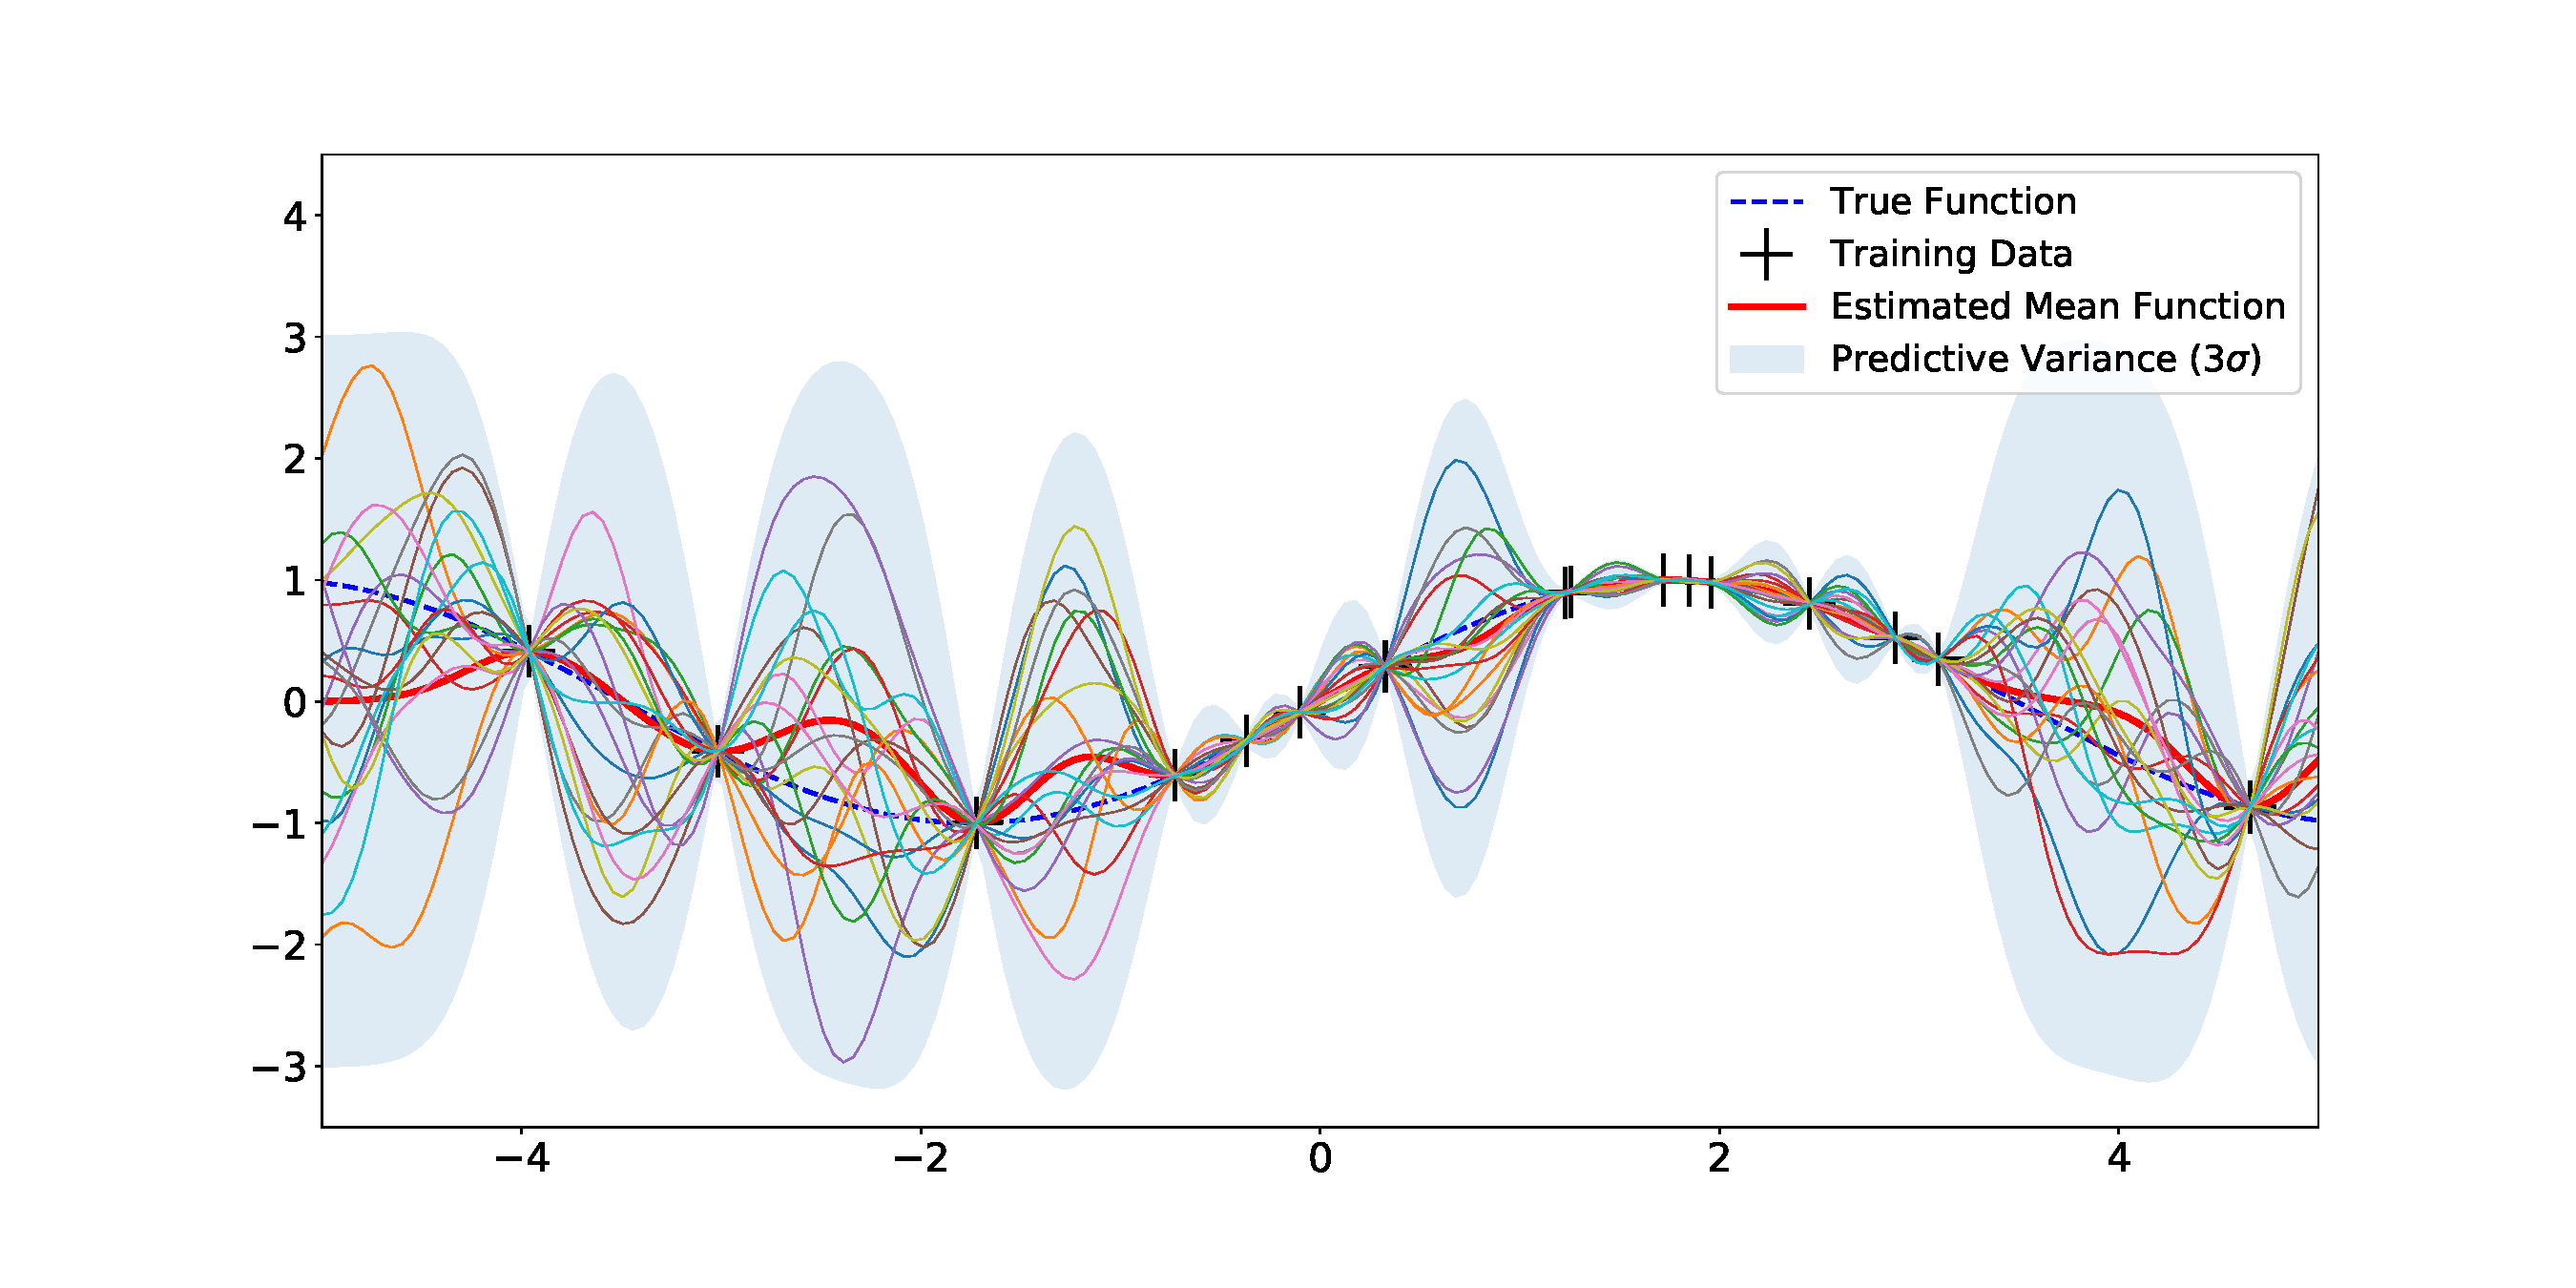
\includegraphics[trim=4.5cm 1.6cm 4.4cm 0.6cm, width=15cm]{figs/illustrative_posterior_func.pdf}}}
	\caption{An example of Gaussian processes regression. The observed data points are generated by the blue dotted line (the true regression function) plotted as black crosses, using the generated data as the observed/training data points, infinite possible posterior functions are obtained. We plotted 20 samples of these infinite functions with sorted colors. The mean function is obtained by the probability distribution of these functions and plotted as a red solid line. The blue shaded area around the mean function indicates the $3\mu$ prediction variance.}
	\label{FIG:10}
\end{figure}

\subsection{Hyperparameters optimization}\label{Hyperparameters}
So far, we talked about the basics and implemented a simple GPR example. While a practical GPR model is more complex than it. The kernel functions play significant roles in GPR. Kernel functions are selected depending on the specific tasks using criteria including if the model is smooth, if it is sparse, if it can change drastically, and if it needs to be differentiable \cite{duvenaud2014automatic}. More information about choosing a kernel/covariance function for a Gaussian processes regression can be found in \cite{duvenaud2014automatic}. 

In kernels, proper hyper-parameters selection are essential. Let's use the most commonly used kernel, RBF, as an example. The general RBF function is 
\begin{ceqn}
    \begin{align}
        k(\mathbf{x}_i,\mathbf{x}_j) = \sigma_f^2 \exp \Big(-\frac{1}{2l^2}
         (\mathbf{x}_i - \mathbf{x}_j)^\mathsf{T}
         (\mathbf{x}_i - \mathbf{x}_j) \Big)  \ , \nonumber
    \end{align}
\end{ceqn}
where $\sigma_f$ and $l$ are hyperparameters \cite{duvenaud2014automatic}. The vertical scale $\sigma_f$ describes how much vertically the function can span. The horizontal scale $l$ indicate how quickly the correlation relationship between two points drops as their distance increase. A higher $l$ provides a smooth function and smaller $l$ results a more wiggly function. The function smoothness affected by $l$ is shown in Fig. \ref{FIG:11}. 
\begin{figure}[h!]
    \centering
    \subfloat[$l$ = small]{{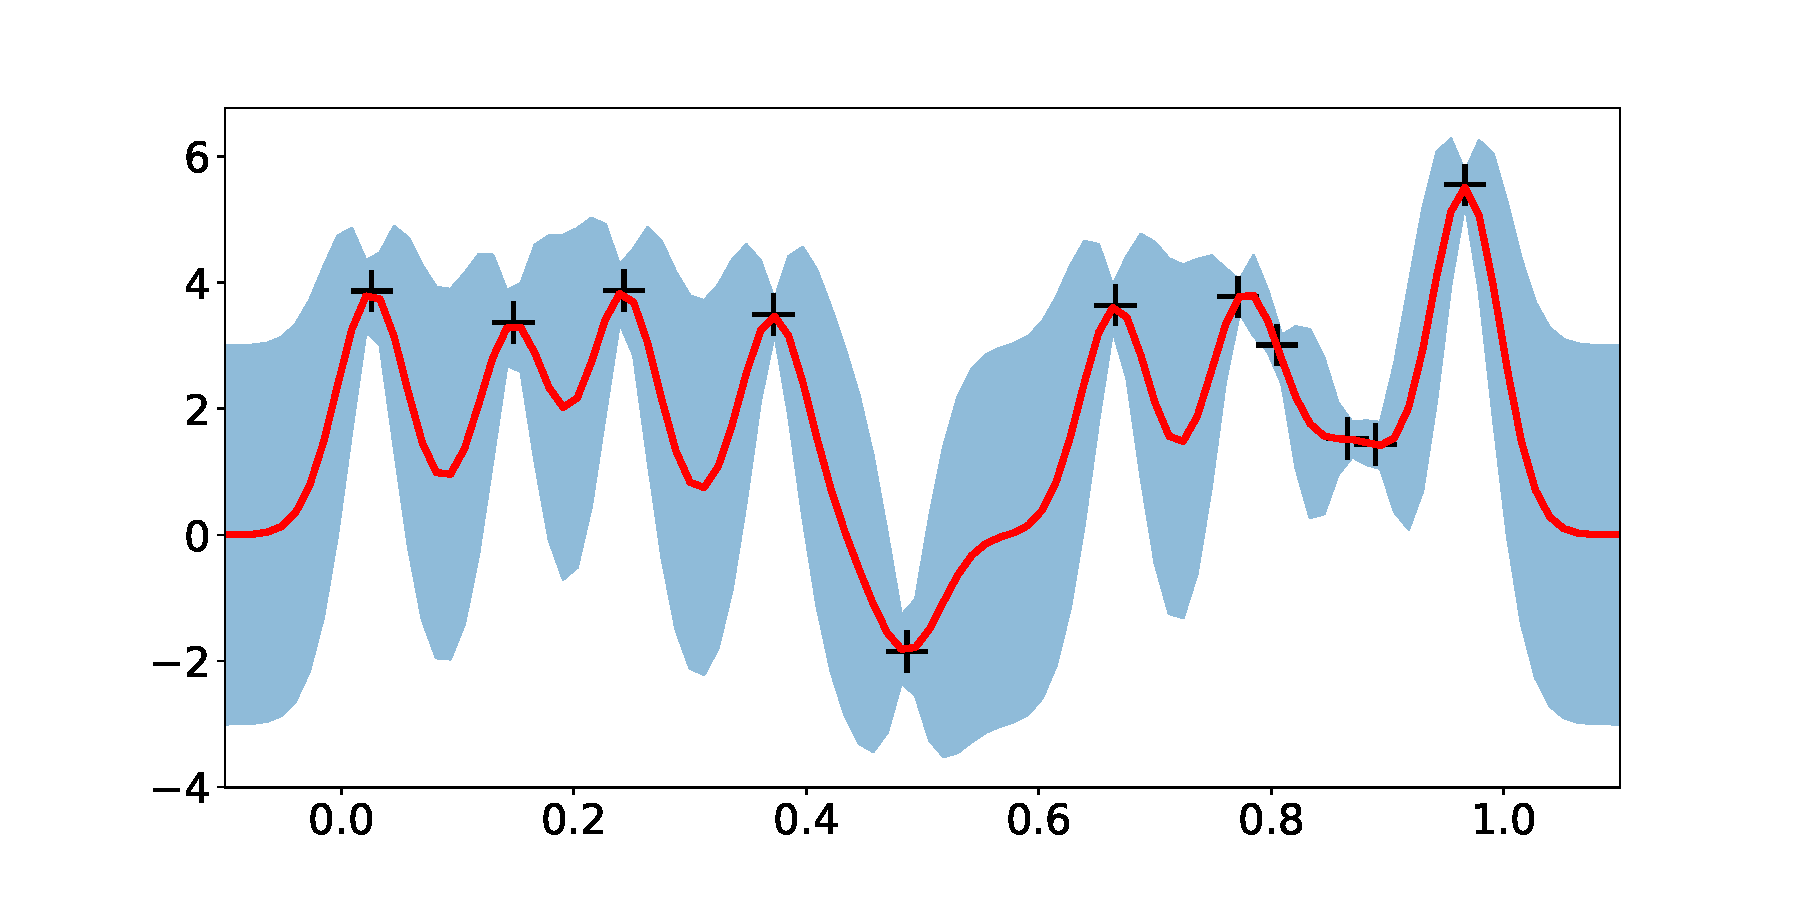
\includegraphics[trim=3.0cm 1.0cm 3.8cm 2cm, width=4.25cm]{figs/l_small.pdf} }}
    \qquad
    \subfloat[$l$ = medium]{{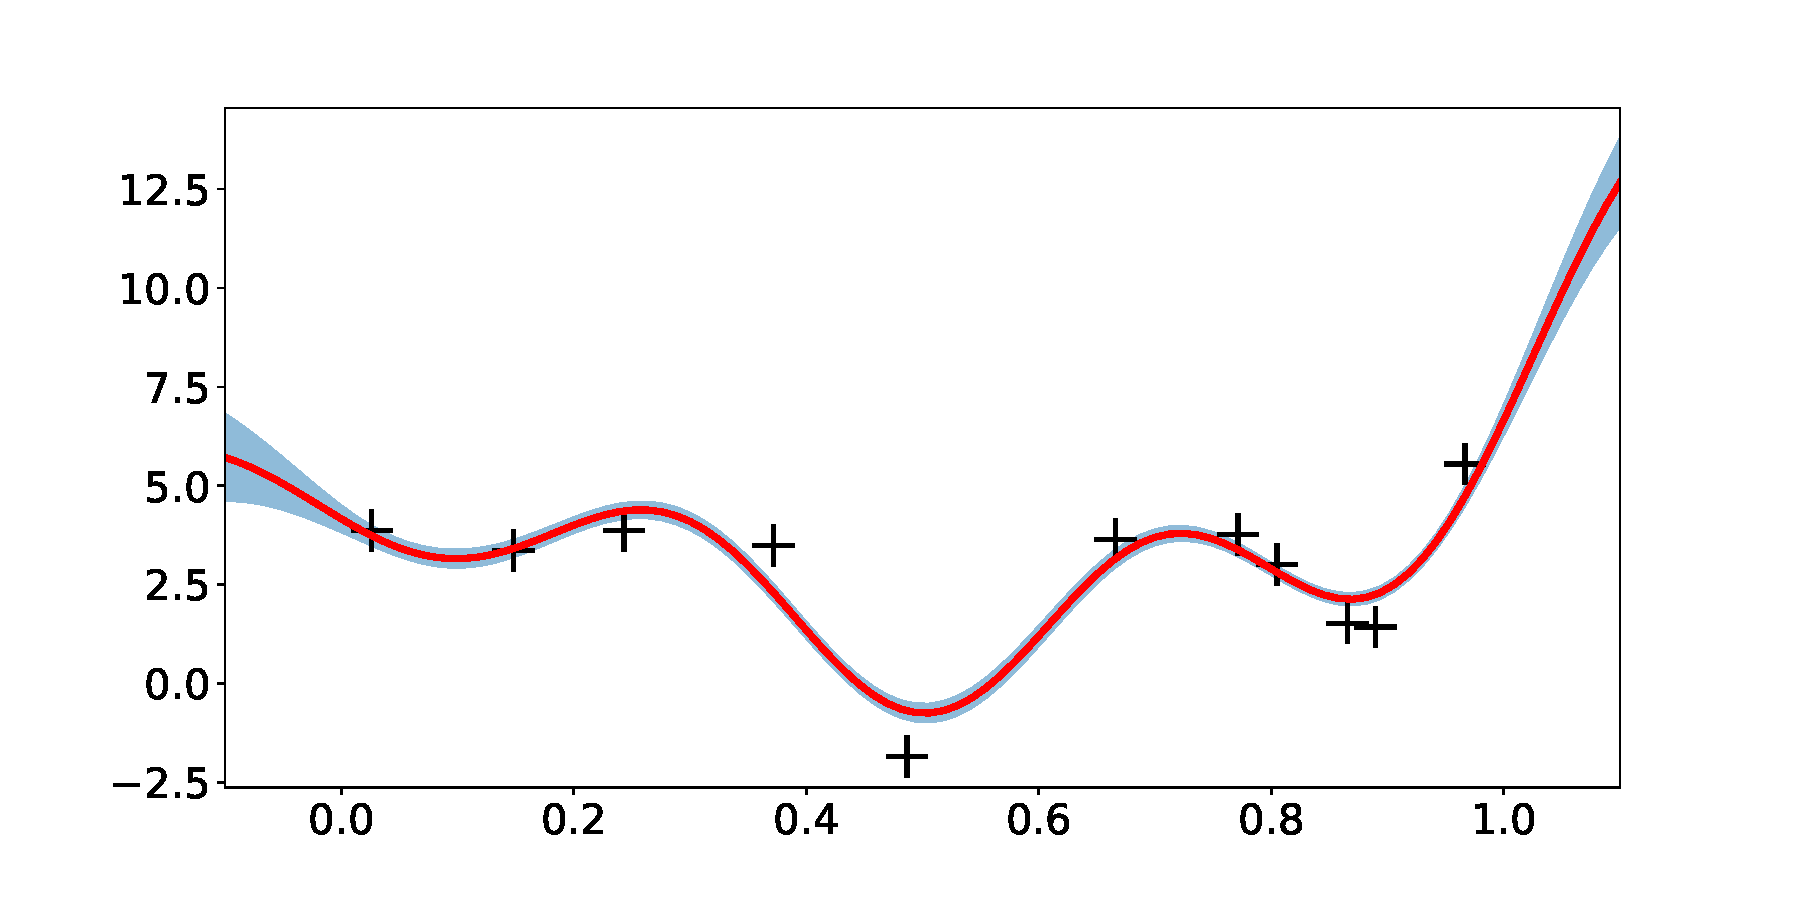
\includegraphics[trim=2.4cm 1.0cm 3.8cm 2cm, width=4.32cm]{figs/l_medium.pdf} }}
    \qquad
    \subfloat[$l$ = large]{{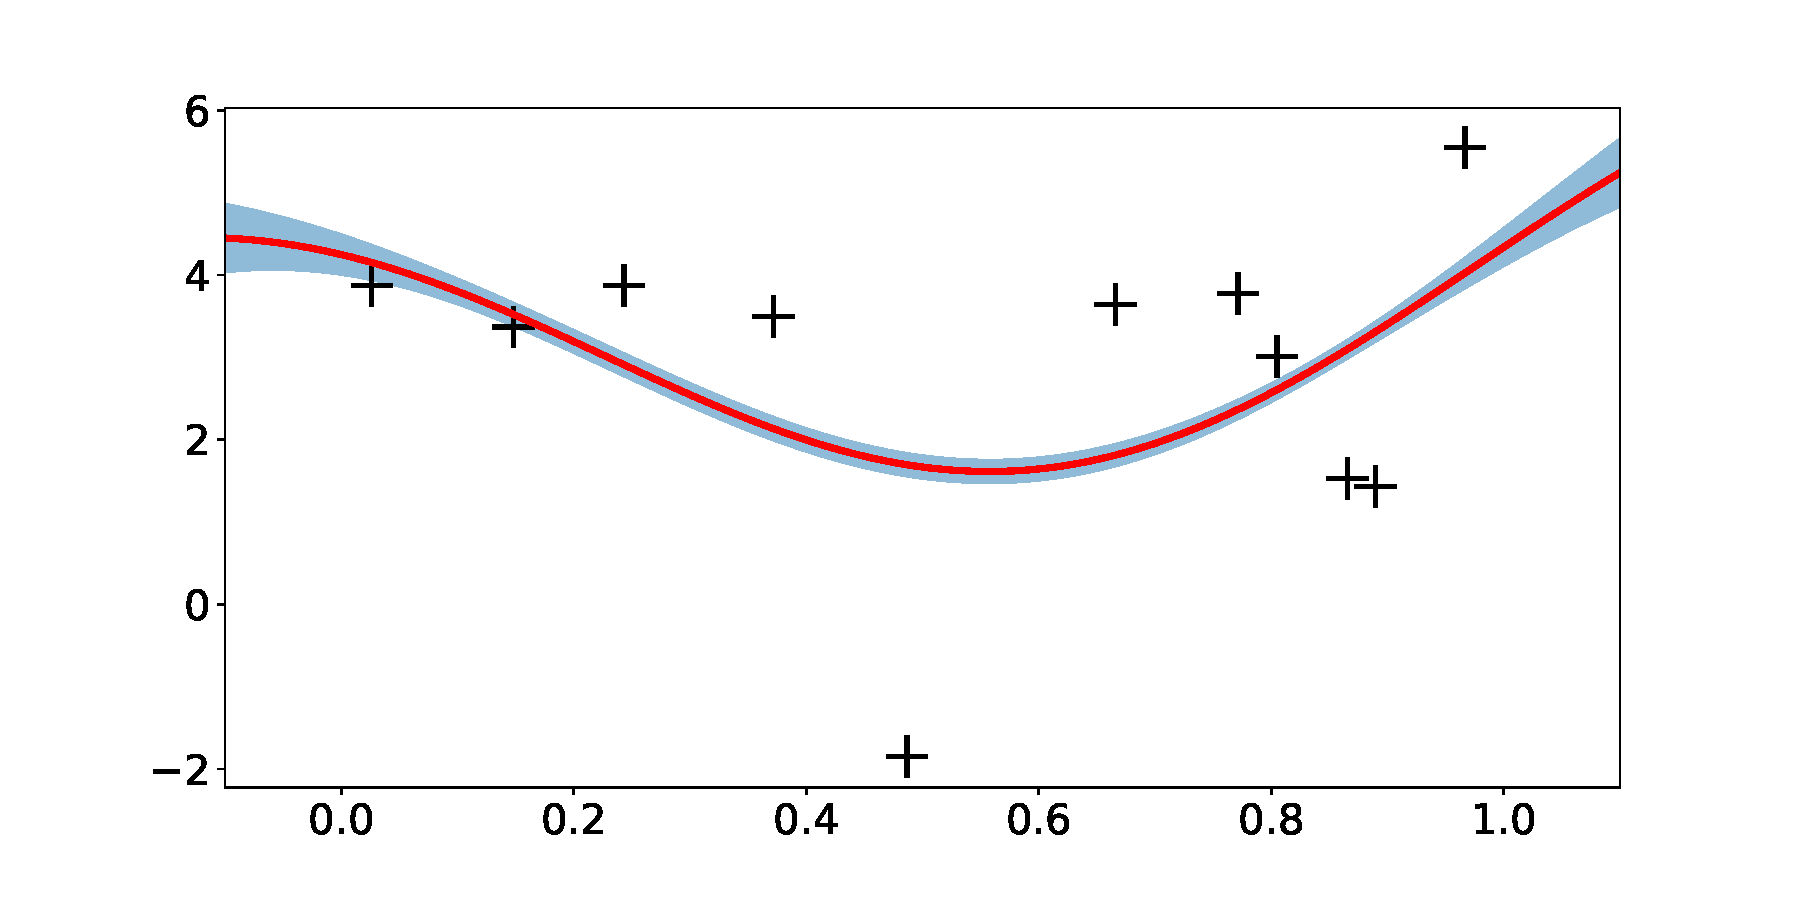
\includegraphics[trim=3.0cm 1.0cm 3.8cm 2cm, width=4.25cm]{figs/l_large.pdf} }}
    \caption{The function smoothness affected by the horizontal scale $l$.}%
    \label{FIG:11}
\end{figure}

The optimized hyperparameters $\boldsymbol {\theta}$ are determined by the Maximum Likelihood Estimate as  
\begin{ceqn}
    \begin{align}
        \boldsymbol {\theta^*} = \arg\max\limits_{\theta} \log p(y \, \vert \, \mathbf{X}, \boldsymbol {\theta})  \ . \nonumber
    \end{align}
\end{ceqn}
Thus, considering hyperparameters optimization, a more general equation of predictions at the testing points is \cite{gpss2019}  
\begin{ceqn}
    \begin{align}
        \mathbf{\bar{f}_*} \, \vert \, \mathbf{X}, \mathbf{y}, \mathbf{X}_*,  \boldsymbol {\theta} \sim \mathcal{N} \left(\mathbf{\bar{f}_*}, \operatorname{cov}(\mathbf{f}_*)\right)  \ . \nonumber
    \end{align}
\end{ceqn}
The regression result of the data points in \ref{FIG:11} with the optimized hyperparameters $\sigma_f = 0.0067$ and $l = 0.0967$ is shown in Fig. \ref{FIG:12}. 

\begin{figure}[h!]
	\centering
		{{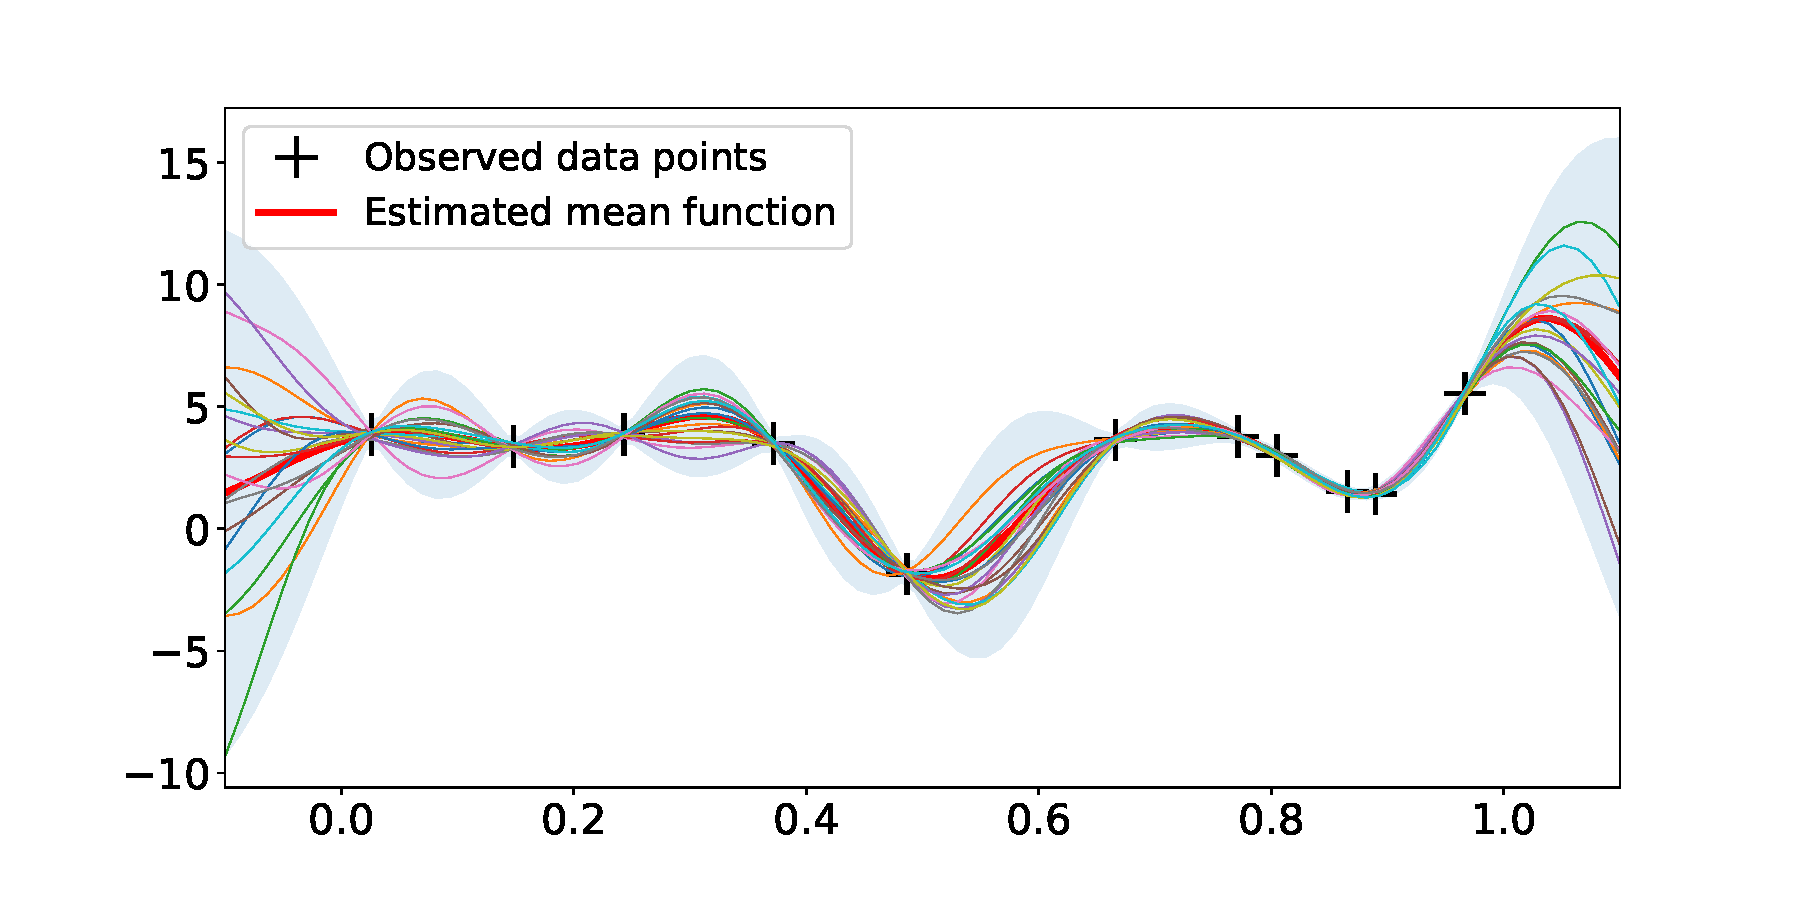
\includegraphics[trim=2.2cm 1.0cm 2.8cm 0.8cm, width=12cm]{figs/regression_gpflow.pdf}}}
	\caption{Regression result with the optimized hyperparameters $\sigma_f$ and $l$.}
	\label{FIG:12}
\end{figure}

\subsection{Gaussian processes packages}
This section reviews three packages written in Python for Gaussian processes implementations. One of the most well-known GP packages is GPy \cite{de2017gpflow}. GPy is a maturely developed package with well-documented explanations since 2012. GPy uses NumPy to perform all its computations. For tasks that don't require heavy computations implementations, GPy is sufficient and stable to use. However, GPR is computationally expensive in high dimensional spaces (features more than a few dozens) due to the fact it uses the whole samples/features to do the predictions. The more observations, the more computations are needed for predictions. A package that includes state-of-the-art algorithms is preferred for efficient implementation of complex GPR tasks. For GPR tasks that are computationally expensive, GPU acceleration is especially useful. GPflow \cite{de2017gpflow} origins from GPy with much of a similar interface. GPflow leverages TensorFlow as its computational backend. GPyTorch \cite{gardner2018gpytorch} is a recently developed package that provides GPU acceleration through PyTorch. It contains very up-to-date GP algorithms. Similar to GPflow, GPyTorch provides automatic gradients. So complex models such as embedding deep neural networks in GP models can be easier developed. 

\section{Summary}
A Gaussian processes model is a probability distribution over possible functions that fit a set of points \cite{Rasmussen2006}. Gaussian process regression provides a distribution with uncertainty estimations for predictions rather than one prediction value. The prior knowledge and specifications about the shape of the function model can be integrated by selecting different kernel functions.

The Gaussian processes format in this introduction is called the standard GP or vanilla GP \cite{frigola2013bayesian}. There are two main constraints with standard Gaussian processes model: 1) The overall computation complexity is $O(N^3)$, where $N$ is the dimension of the covariance matrix $K$. 2) The memory consumption is quadratic. Because of the computation complexity and memory consumption, the standard Gaussian processes model gets struck quickly. For regression tasks with a big dataset, sparse GP is used to reduce computational complexity \cite{frigola2013bayesian}.

\appendix
\section{Appendix}
\label{APPENDIX}

The Marginal and conditional distributions of MVN theorem: suppose $X=({x}_1,{x}_2)$ is jointly Gaussian with parameters
\begin{ceqn}
    \begin{align}
        {\mu}=\begin{bmatrix}{\mu}_1 \\ {\mu}_2\end{bmatrix} , \ 
        {\Sigma}=\begin{bmatrix} {\Sigma}_{11} & {\Sigma}_{12} \\ {\Sigma}_{21} & {\Sigma}_{22} \end{bmatrix} , \ 
        {\Lambda}={\Sigma}^{-1}=\begin{bmatrix} {\Lambda}_{11} & {\Lambda}_{12} \\ {\Lambda}_{21} & {\Lambda}_{22} \end{bmatrix} \ , \nonumber
    \end{align}
\end{ceqn}
then the marginals are given by
\begin{ceqn}
    \begin{equation}
        \begin{split}
            p({x}_1)= \mathcal{N}({x}_1|{\mu}_1,{\Sigma}_{11}) \ , \\
            p({x}_2)= \mathcal{N}({x}_2|{\mu}_2,{\Sigma}_{22})  \ , \nonumber
        \end{split}
    \end{equation}
\end{ceqn}
and the posterior conditional is given by

\begin{ceqn}
   \begin{equation}\label{eqn:Marginals-and-conditionals-of-an-MVN}
       \boxed{\begin{split}
        p({x}_1|{x}_2)& =\mathcal{N}({x}_1|{\mu}_{1|2},{\Sigma}_{1|2}) \\
        {\mu}_{1|2}& = {\mu}_1+{\Sigma}_{12}{\Sigma}_{22}^{-1}({x}_2-{\mu}_2) \\
    	               & = {\mu}_1-{\Lambda}_{11}^{-1}{\Lambda}_{12}({x}_2-{\mu}_2) \\
    				   & = {\Sigma}_{1|2}({\Lambda}_{11}{\mu}_1-{\Lambda}_{12}({x}_2-{\mu}_2)) \\
    	{\Sigma}_{1|2}& = {\Sigma}_{11}-{\Sigma}_{12}{\Sigma}_{22}^{-1}{\Sigma}_{21}={\Lambda}_{11}^{-1} \nonumber
       \end{split}}
    \end{equation}
\end{ceqn}

%% Loading bibliography style file
\bibliographystyle{plain}
% Loading bibliography database
\bibliography{bibliography}



\end{document}

